% ------ | ------- | ------- | ------- | ------- | ------- | ------- | ------- |
%
\documentclass[twocolumn,twoside,fleqn,12pt]{article}
%
% This lightly writes DRAFT across each page.
\usepackage{draftcopy}
%
% Handling footnotes
\usepackage{ftnright}                  % Places footnotes in right column
\setlength{\skip\footins}{8pt}         % Sets footnote size to 8pt
\addtolength{\textheight}{1in}         % Adjusts spacing for footnotes
\preparefootins                        % Saves these parameters
%
% For handling encapsulated postscript files.
\usepackage[pdftex]{graphicx}
%\usepackage{epsfig}
%
% Single column figure
%\begin{figure}
%   \centering
%   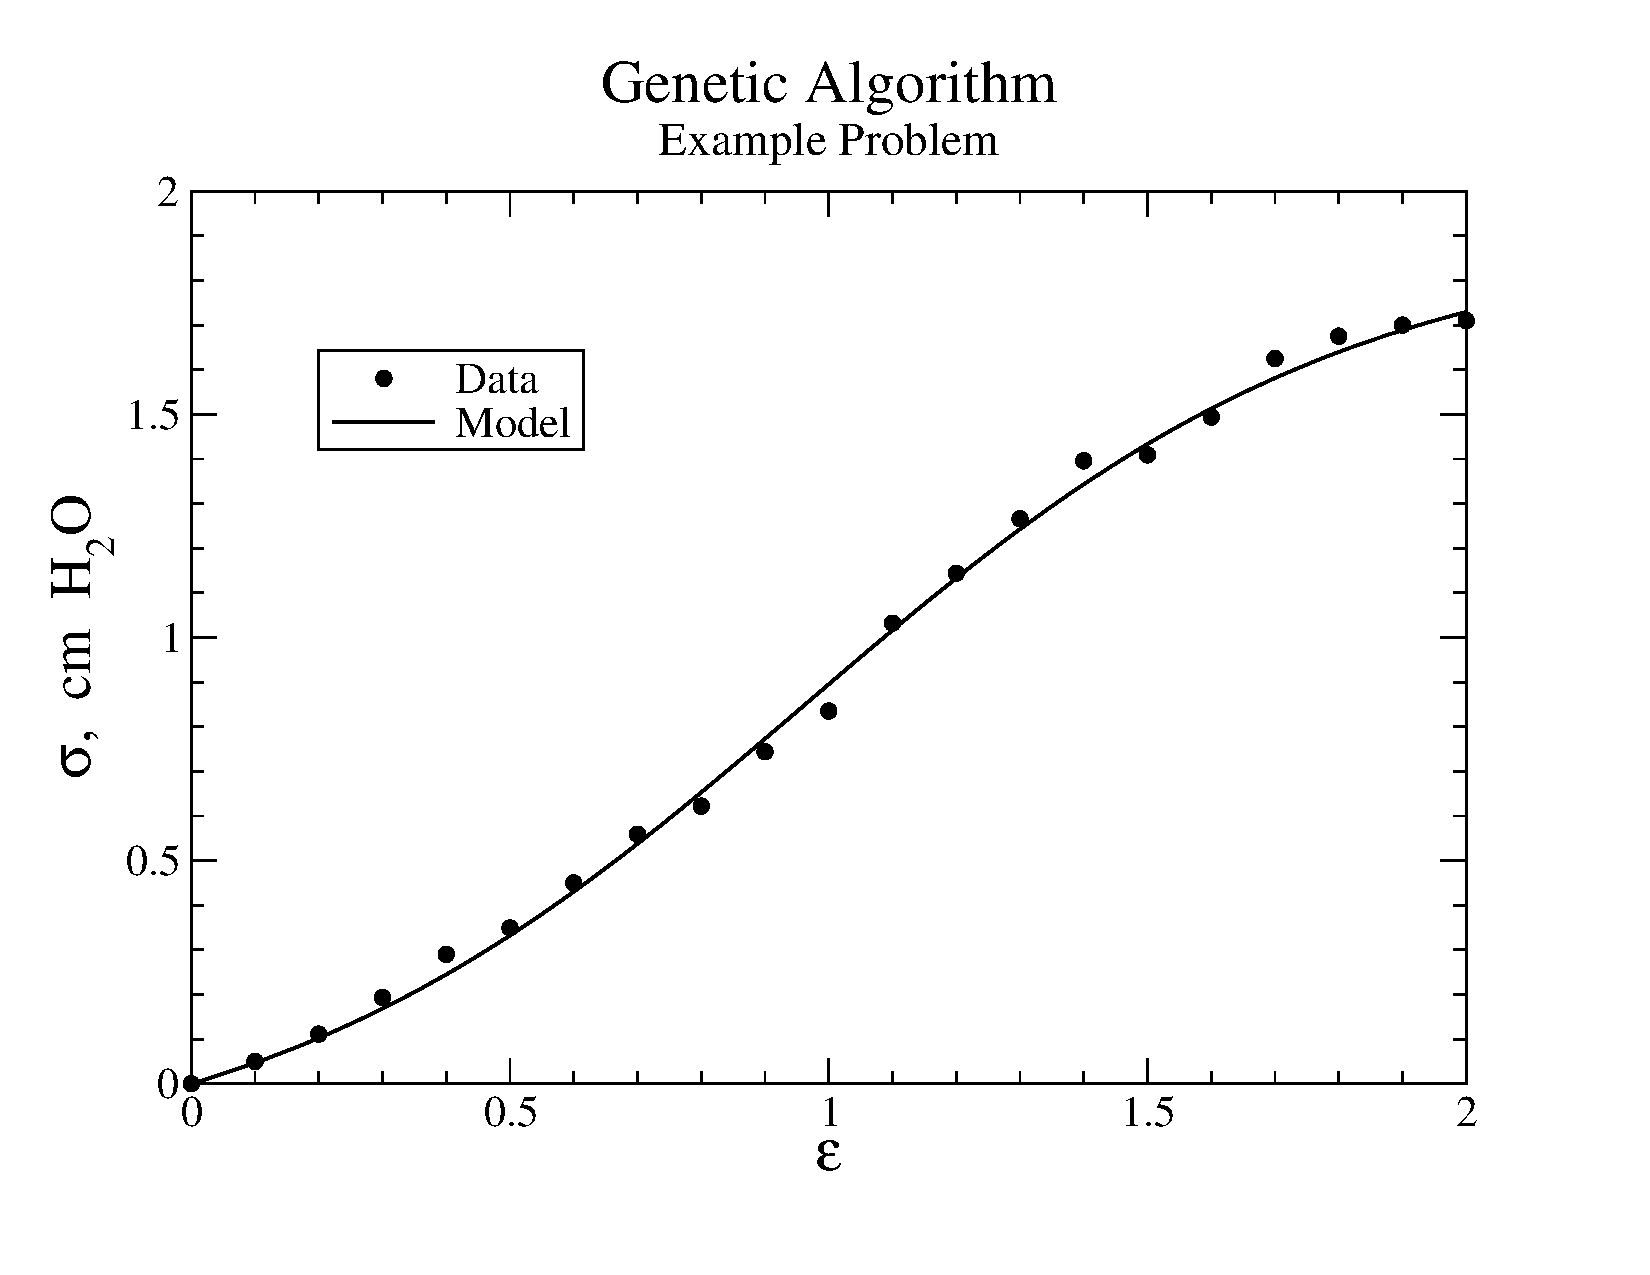
\includegraphics[angle=-90,width=8cm]{gaExample.pdf}
%   \caption{...}
%   \label{...}
%\end{figure}
%
% Double column figure
%\begin{figure*}
%   {\par\centering
%   \resizebox*{1.0\textwidth}{.25\textheight}
%   {\includegraphics[angle=-90]{<figure.eps>}}
%   \par}
%   \caption{\label{<figureLabel>}%
%   }
%\end{figure*}
%
% Tables are the same. A one column table has the structure
%\begin{table}
%  ...
%\end{table}
%
% while a two-column table is created with
%\begin{table*}
%  ...
%\end{table*}
%
%
% Set up babel for typesetting bibliographies.
\usepackage[english]{babel}  %language selection
\selectlanguage{english}
% Languages supported by babel include:
%   american, austrian, brazil, catalan, croatian, czech, danish, dutch,
%   english, esperanto, finnish, french, galician, german, italian, magyar,
%   norsk, nynorsk, polish, portuges, romanian, russian, slovak, slovene,
%   spanish, swedish, turkish.
%
% Select the default text font which is used, for example,
% in the typesetting of the front matter of a paper
% and in the typesetting text in formulae, e.g., sin.
% The Monotype Baskerville fonts are sold separately at: http://www.fonts.com.
%\renewcommand{\rmdefault}{cmr}        % computer modern roman
%\renewcommand{\rmdefault}{txr}        % TX fonts
%\renewcommand{\rmdefault}{ptm}        % Adobe times roman
%\renewcommand{\rmdefault}{mbv}        % Baskerville with inline numbers
\renewcommand{\rmdefault}{mbvj}        % Baskerville with old-style numbers
%
% If AMS-LaTeX macros are to used, load them before mtpro.
% MTPro will replace the AMS fonts, but not its macros.
\usepackage{amsmath, amsthm}
%
% Load MathTime Professional II fonts - commercial fonts
% For sales and other information visit www.pctex.com.
% The following math fonts are created:
%   \mathrm   \mathit    \mathsf   \mathtt
%   \mathbf   \mathbold  \mbf      \mathbb
%   \mathcal  \mathbcal  \mathscr  \mathbscr  \mathfrak
%\usepackage[subscriptcorrection,slantedGreek,boldalphabet,mtpccal,mtpscr,mtpfrak,mtphrb,zswash,nofontinfo]{mtpro2}
\usepackage[subscriptcorrection,slantedGreek,mtpccal,mtpscr,mtpfrak,mtphrb,zswash,nofontinfo]{mtpro2}
%
% Introduce the text fonts.
%
% Define a set of macros for characterizing text fonts.
%   medium fonts   roman     san serif    typewriter
%     upright     \fontrm    \fontss      \fonttt
%     slant       \fontsl    \fontsssl    \fontttsl
%     small cap   \fontsc    \fontsssc    \fontttsc
%     italic      \fontit
%
%   bold fonts     roman     san serif    typewriter
%     upright     \boldrm    \boldss      \boldtt
%     slant       \boldsl    \boldsssl    \boldttsl
%     small cap   \boldsc    \boldsssc    \boldttsc
%     italic      \boldit
%
% Establish the default font encoding scheme to use.
\DeclareFontEncoding{T1}{}{}           % specify text font encoding scheme
\DeclareFontEncoding{TS1}{}{}          % specify text companion font encoding
%
% Normal text fonts.
\DeclareFontFamily{T1}{txr}{\hyphenchar\font=127}
\DeclareFontShape{T1}{txr}{m}{n}{<-> t1xr}{}
\DeclareFontShape{T1}{txr}{m}{sl}{<-> t1xsl}{}
\DeclareFontShape{T1}{txr}{m}{sc}{<-> t1xsc}{}
\DeclareFontShape{T1}{txr}{m}{it}{<-> t1xi}{}
\renewcommand{\normalfont}{\usefont{T1}{txr}{m}{n}}
\newcommand{\fontrm}[1]{\normalfont{#1}}
\newcommand{\fontsl}[1]{\usefont{T1}{txr}{m}{sl}{#1}\normalfont}
\newcommand{\fontsc}[1]{\usefont{T1}{txr}{m}{sc}{#1}\normalfont}
\newcommand{\fontit}[1]{\usefont{T1}{txr}{m}{it}{#1}\normalfont}
%
% Bold text fonts.
\DeclareFontFamily{T1}{txb}{\hyphenchar\font=127}
\DeclareFontShape{T1}{txb}{bx}{n}{<-> t1xb}{}
\DeclareFontShape{T1}{txb}{bx}{sl}{<-> t1xbsl}{}
\DeclareFontShape{T1}{txb}{bx}{sc}{<-> t1xbsc}{}
\DeclareFontShape{T1}{txb}{bx}{it}{<-> t1xbi}{}
\newcommand{\boldrm}[1]{\usefont{T1}{txb}{bx}{n}{#1}\normalfont}
\newcommand{\boldsl}[1]{\usefont{T1}{txb}{bx}{sl}{#1}\normalfont}
\newcommand{\boldsc}[1]{\usefont{T1}{txb}{bx}{sc}{#1}\normalfont}
\newcommand{\boldit}[1]{\usefont{T1}{txb}{bx}{it}{#1}\normalfont}
%
% Normal san serif fonts.
\DeclareFontFamily{T1}{txss}{\hyphenchar\font=127}
\DeclareFontShape{T1}{txss}{m}{n}{<-> s * [0.95] t1xss}{}
\DeclareFontShape{T1}{txss}{m}{sl}{<-> s * [0.95] t1xsssl}{}
\DeclareFontShape{T1}{txss}{m}{sc}{<-> s * [0.95] t1xsssc}{}
\newcommand{\fontss}[1]{\usefont{T1}{txss}{m}{n}{#1}\normalfont}
\newcommand{\fontsssl}[1]{\usefont{T1}{txss}{m}{sl}{#1}\normalfont}
\newcommand{\fontsssc}[1]{\usefont{T1}{txss}{m}{sc}{#1}\normalfont}
%
% Bold san serif fonts.
\DeclareFontFamily{T1}{txssb}{\hyphenchar\font=127}
\DeclareFontShape{T1}{txssb}{bx}{n}{<-> s * [0.95] t1xbss}{}
\DeclareFontShape{T1}{txssb}{bx}{sl}{<-> s * [0.95] t1xbsssl}{}
\DeclareFontShape{T1}{txssb}{bx}{sc}{<-> s * [0.95] t1xbsssc}{}
\newcommand{\boldss}[1]{\usefont{T1}{txssb}{bx}{n}{#1}\normalfont}
\newcommand{\boldsssl}[1]{\usefont{T1}{txssb}{bx}{sl}{#1}\normalfont}
\newcommand{\boldsssc}[1]{\usefont{T1}{txssb}{bx}{sc}{#1}\normalfont}
%
% Normal typewriter fonts.
\DeclareFontFamily{T1}{txtt}{\hyphenchar\font=127}
\DeclareFontShape{T1}{txtt}{m}{n}{<-> t1xtt}{}
\DeclareFontShape{T1}{txtt}{m}{sl}{<-> t1xttsl}{}
\DeclareFontShape{T1}{txtt}{m}{sc}{<-> t1xttsc}{}
\newcommand{\fonttt}[1]{\usefont{T1}{txtt}{m}{n}{#1}\normalfont}
\newcommand{\fontttsl}[1]{\usefont{T1}{txtt}{m}{sl}{#1}\normalfont}
\newcommand{\fontttsc}[1]{\usefont{T1}{txtt}{m}{sc}{#1}\normalfont}
%
% Bold typewriter fonts.
\DeclareFontFamily{T1}{txttb}{\hyphenchar\font=127}
\DeclareFontShape{T1}{txttb}{bx}{n}{<-> t1xbtt}{}
\DeclareFontShape{T1}{txttb}{bx}{sl}{<-> t1xbttsl}{}
\DeclareFontShape{T1}{txttb}{bx}{sc}{<-> t1xbttsc}{}
\newcommand{\boldtt}[1]{\usefont{T1}{txttb}{bx}{n}{#1}\normalfont}
\newcommand{\boldttsl}[1]{\usefont{T1}{txttb}{bx}{sl}{#1}\normalfont}
\newcommand{\boldttsc}[1]{\usefont{T1}{txttb}{bx}{sc}{#1}\normalfont}
%
\usepackage{xspace} % provides appropriate spacing
% Redefine the standard text font selecting macros.
\renewcommand{\textrm}[1]{\fontrm{#1}\xspace}
\renewcommand{\textbf}[1]{\boldrm{#1}\xspace}
\renewcommand{\textit}[1]{\fontit{#1}\xspace}
\renewcommand{\textsc}[1]{\fontsc{#1}\xspace}
\renewcommand{\textsf}[1]{\fontss{#1}\xspace}
\renewcommand{\textsl}[1]{\fontsl{#1}\xspace}
\renewcommand{\texttt}[1]{\fonttt{#1}\xspace}
\renewcommand{\textup}[1]{\fontrm{#1}\xspace}
% If xspace provides unwanted spacing, do not use the
% base \font## or \bold## commands instead of \text##.
%
\newcommand{\eg}{e.g.,\xspace}
\newcommand{\ie}{i.e.,\xspace}
\newcommand{\viz}{viz.,\xspace}
\newcommand{\cf}{cf.\@\xspace}
\newcommand{\eq}{Eq.\@\xspace}
\newcommand{\eqs}{Eqs.\@\xspace}
\newcommand{\etc}{etc.\@\xspace}
\newcommand{\fig}{Fig.\@\xspace}
\newcommand{\figs}{Figs.\@\xspace}
\newcommand{\vs}{vs.\@\xspace}
%
% For underlining options
%\usepackage{ulem}
%    \uline{important}   underlined text
%    \uuline{urgent}     double-underlined text
%    \uwave{boat}        wavy underline
%    \sout{wrong}        line drawn through word
%    \xout{removed}      marked over with //////
%
% Define macros for writing tensor equations.
%
% Macro for typesetting numbers in text.
\newcommand{\scalar}[1]%
   {\fontencoding{TS1}\selectfont #1\fontencoding{T1}\selectfont}
%
% Macros for typesetting vectors - italic roman.
\DeclareMathAlphabet{\mathitbb}{U}{mt2hrb}{m}{it}
\newcommand{\vecFld}[1]{\ensuremath{\mathbold{#1}}}
\newcommand{\vecEle}[1]{\ensuremath{\mathit{#1}}}
\newcommand{\vecMtx}[1]{\ensuremath{\mathitbb{#1}}}
%
% Macros for typesetting tensors of second rank - upright roman.
\newcommand{\tenFld}[1]{\ensuremath{\mbf{#1}}}
\newcommand{\tenEle}[1]{\ensuremath{\mathrm{#1}}}
\newcommand{\tenMtx}[1]{\ensuremath{\mathbb{#1}}}
%
% Macros for typesetting tensors of fourth rank - italic san serif.
\DeclareMathAlphabet{\mathsfbb}{U}{mt2bb}{m}{it}
\newcommand{\TenFld}[1]{\ensuremath{\text{\boldsssl{#1}}}}
\newcommand{\TenEle}[1]{\ensuremath{\text{\fontsssl{#1}}}}
\newcommand{\TenMtx}[1]{\ensuremath{\mathsfbb{#1}}}
%
% Macros for typesetting greek symboled fields.
\newcommand{\grkFld}[1]{\ensuremath{\mathbold{#1}}}
\newcommand{\grkEle}[1]{\ensuremath{#1}}
\newcommand{\grkMtx}[1]{\ensuremath{\mathitbb{#1}}}
%
% Macros for creating nice text and script fractions.
%   There is a cleaner way to do this; for example,
%   \newcommand*{\textfrac}[2]{%
%      {\fontfamily{<fontname>1}\selectfont #1}%
%      \textfractionsolidus
%      {\fontfamily{<fontname>0}\selectfont #2}}%
%   See http://www.ctan.org/tex-archive/macros/latex/doc/fntguide.pdf
%   Sec. V.5: Using the feature of expert fonts
%   Here we must use the following hack because Adobe Times Roman and
%   Baskerville expert fonts do not contain the superior <fontname>1
%   and inferior <fontname>0 glyphs in their font tables.
% Do not break these long lines into multiple lines
% Spaces CANNOT be present - they cause unwanted `rubber' spacing
\newcommand{\textfrac}[2]
   {\leavevmode
    \kern.05em\raise.6ex\hbox{\ensuremath{\scriptstyle{#1}}}\kern-.05em\hspace{0em}/\hspace{0em}\kern-.05em\lower.2ex\hbox{\ensuremath{\scriptstyle{#2}}}\kern.05em
   }
\newcommand{\scriptfrac}[2]
   {\leavevmode
    \kern.05em\raise.3ex\hbox{\ensuremath{\scriptscriptstyle{#1}}}\kern-.05em\hspace{0em}\hbox{\ensuremath{\scriptstyle{/}}}\hspace{0em}\kern-.05em\lower.25ex\hbox{\ensuremath{\scriptscriptstyle{#2}}}\kern.05em
   }
%
% Layout and formatting of the document.
%
% Macro used for creating nomenclatures, etc.
\newcommand{\namelistlabel}[1]{\mbox{#1}\hfil}
\newenvironment{namelist}[1]
   {\begin{list}{}%
      {\let\makelabel\namelistlabel%
       \settowidth{\labelwidth}{#1}%
       \setlength{\leftmargin}{1.1\labelwidth}%
       \setlength{\itemsep}{-6pt}%
      }%
   }{\end{list}%
}
%
% page size
\pdfpagewidth 8.5in
\pdfpageheight 11in
% top margin
\setlength\topmargin{-0.25in}
% header properties
\setlength\headheight{0in}
\setlength\headsep{0in}
% printed size on paper
\setlength\textheight{9.5in}
\setlength\textwidth{7in}
% margins for two-sided printing
\setlength\oddsidemargin{0in}
\setlength\evensidemargin{-0.4in}
% paragraph properties
\setlength\parindent{0.25in}
\setlength\parskip{0.05in}
% Column separation
\setlength{\columnsep}{15pt}
\setlength{\columnseprule}{0pt}
% Fill page
\flushbottom
%
%
% don't hyphenate so much - default = 200, max (never hyphenate) = 10,000
\hyphenpenalty=800
%
% two column float page must be 90% full
\renewcommand\dblfloatpagefraction{.90}
% two column top float can cover up to 80% of page
\renewcommand\dbltopfraction{.80}
% float page must be 90% full
\renewcommand\floatpagefraction{.90}
% top float can cover up to 80% of page
\renewcommand\topfraction{.80}
% bottom float can cover up to 80% of page
\renewcommand\bottomfraction{.80}
% at least 10% of a normal page must contain text
\renewcommand\textfraction{.1}
%
% separation between floats and text
\setlength\dbltextfloatsep{9pt plus 5pt minus 3pt }
% separation between two column floats and text
\setlength\textfloatsep{10pt plus 4pt minus 3pt}
%
%
% Additional declarations beyond my standard template.
%
%  A phantom minus sign used for alignment in tables, etc.
\def\m{\phantom{-}}
%
%%%%%%%%%%%%%%%%%%%%%%%%%%%%%%%%%%%%%%%%%%%%%%%%%%
%
%
%
\begin{document}
%
\bibliographystyle{asme}       % numeric bibliography format
%\bibliographystyle{plain}
%
\title{\textsf{BEL}--Math\\
       A \textsf{.NET} Computational Package Written in Zonnon\\
       Part III of the Users Guide\\
       \phantom{A}}
%
\author{Alan D.\ Freed\\
\and
\mbox{}\hfill Clifford H.\ Spicer Chair in Engineering\\
\mbox{}\hfill College of Science, Engineering \& Technology\\
\mbox{}\hfill Saginaw Valley State University\\
\mbox{}\hfill 202 Pioneer Hall, 7400 Bay Road\\
\mbox{}\hfill University Center, MI 48710\\
\mbox{}\hfill E-Mail: \texttt{adfreed@svsu.edu}\\
}
%
\date{\today}



\maketitle
\normalfont


\begin{figure}
   \centering
   
\includegraphics[width=8cm]{BelLogo.pdf}
\end{figure}

\begin{abstract}
This document describes some useful math modules that are part of the
\textsf{BEL} software library written in the \textsf{Zonnon} programming
language for the \textsf{.NET} and \textsf{Mono} frameworks.
\textsf{BEL} provides a simple, computational, programming interface that
resides on top of \textsf{Zonnon}. Its purpose is to assist in rapid
program development, specifically in the area of computational
continuum mechanics, by leveraging the wide diversity of existing
\textsf{.NET} and \textsf{Mono} libraries with the simple, logical
constructs of the \textsf{Zonnon} programming language.
\end{abstract}


\section{Introduction}
\label{introSection}

\textsf{BEL} is an acronym taken for my research laboratory: The Biological
Engineering Laboratory at Saginaw Valley State University. What \textsf{BEL}
is and what it provides are quite different from what one might expect,
given this affiliation. \textsf{BEL} arose out of the author's desire to
interface with the \textsf{.NET} and \textsf{Mono} Frameworks for the purpose
of writing computational software programs in the \textsf{Zonnon} programming
language \cite{Zonnon09,Zonnon10}.

\textsf{Zonnon} is the most recent descendant from the family
tree \textsf{Euler}\slash \textsf{Algol}\slash \textsf{Pascal}\slash
\textsf{Modula}\slash \textsf{Oberon} of programming languages
developed by Profs.\ \textsc{Niklaus Wirth} and \textsc{J\"urg Gutknecht}
from the Computer Systems Institute at ETH Zurich (Eidgen\"ossische
Technische Hochschule, Zentrum, \ie the Swiss Federal Institute of
Technology, Zurich).  \textsf{Zonnon} was created specifically for
\textsf{.NET}, with compiler versions available for both the \textsf{.NET}
and \textsf{Mono} Frameworks. Sponsored by Xamarin, Mono is an open 
source implementation of Microsoft's .NET Framework based on the 
ECMA standards for C\# and the Common Language Runtime.
The \textsf{Zonnon} compiler targets the \textsf{.NET} 
Framework~2.0.

The \textsf{Zonnon} compiler, documentation, example programs, 
and even \textsf{BEL} itself, are free to download
from \texttt{http:\slash\slash www.zonnon.ethz.ch}.
The home page for Microsoft's \textsf{.NET} Framework is at
\texttt{http:\slash\slash www.microsoft.com\slash net}.
\textsf{Mono}'s is at
\texttt{http:\slash\slash www.mono-project.com\slash Main_Page}.

Licensing of the \textsf{BEL} library, both its software and
documentation, is addressed in the \textit{Licensing of the
Software and its Documentation\/} part to this user guide.


\subsection{Version}

This document corresponds to software version 4.2 of \textsf{BEL-Math},
\today.  \textsf{Zonnon} targets the \textsf{.NET} Framework~2.


\subsection{Required Libraries}

The only external library that is required to compile \textsf{BEL-Math} is 
the one that you created when you built \textsf{BEL}.  When compiling
\textsf{Bel-Math} it is important to place file \texttt{interpolations.znn} 
first in the list of files because it exports types that are used by 
the other files in this library.


\subsection{Known Issues}

There are no know issues regarding \textsf{BEL-Math}.  Having
said this, of all the libraries in the \textsf{BEL} suite,
this is the one most likely to be added to over time.  One is
always running into new math techniques, algorithms, solvers,
\etc that will warrant their addition to this library.


\subsection{Feedback}

I consider this to be a living document. If there is some aspect that is
wanting, or if you have corrections and/or additions that you believe
would benefit other users of \textsf{BEL-Math}, please forward them to
\texttt{adfreed@svsu.edu}.


\section{Mathematics}

\textsf{BEL} contains a modest set of math libraries.  They are split
into two topical regimes: functions and the calculus.
Their interfaces are provided in App.~\ref{mathAppendix}.  The basic
trigonometric, logarithmic, and hyperbolic functions reside in module
\textsf{Bel.Math}, which is now part of the core \textsf{BEL} library.

The author has written a variety of other math procedures in \textsf{Oberon}
that he would like to port over to \textsf{BEL-Math} in future releases.


\subsection{Special Functions}

Module \texttt{BelMath.SpecialFunctions} provides a variety of 
math functions that are more specialized than one would find in 
a typical math library, which are otherwise found in \texttt{Bel.Math}. 
The special functions in this library are:

\noindent Procedure \texttt{Erf} returns the error function of 
its argument.  The error function $\mathrm{erf}(x)$ is defined by
\begin{displaymath}
   \mathrm{erf} (x) = \frac{2}{\sqrt{\pi}} \int_0^x 
   \mathrm{e}^{-y^2} \, \mathrm{d} y
\end{displaymath}
with a graphical presentation displayed in Fig.~\ref{erfFig}.

\begin{figure}
   \centering
   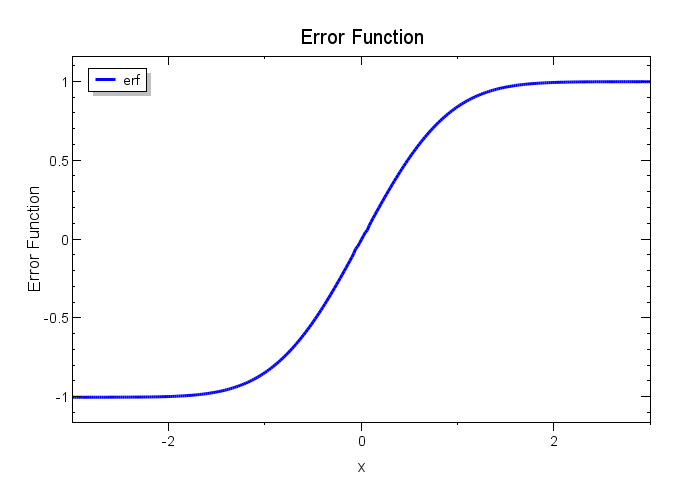
\includegraphics[width=8cm]{erfFn.png}
   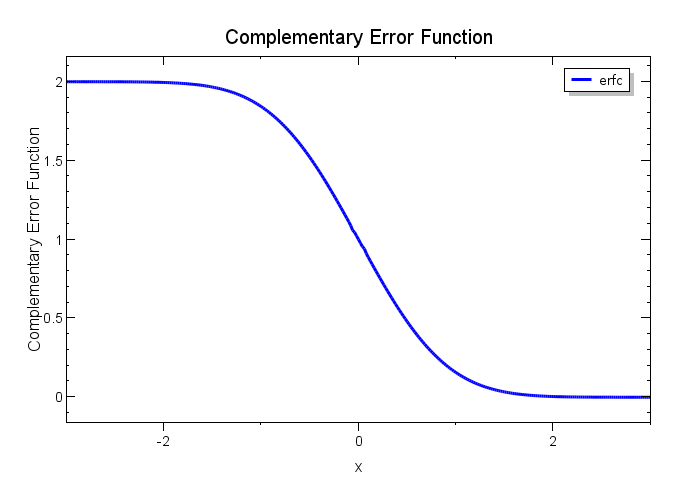
\includegraphics[width=8cm]{erfcFn.png}
   \caption{The error function is on top.  The complementary error 
      function is below.}
   \label{erfFig}
\end{figure}

\noindent Procedure \texttt{Erfc} returns the complimentary 
error function of its argument.  The complementary error function 
$\mathrm{erfc}(x)$ obeys
\begin{displaymath}
   \mathrm{erf}(x) + \mathrm{erfc}(x) = 1 
\end{displaymath}
with a graphical presentation displayed in Fig.~\ref{erfFig}.

\noindent Procedure \texttt{Gamma} returns the gamma function 
of its argument. The gamma function $\Gamma (x)$ is defined by 
\begin{equation*}
   \Gamma (x) = \int_0^{\infty} y^{x-1} \mathrm{e}^{-y} \, 
   \mathrm{d} y
\end{equation*}
with a graphical presentation displayed in Fig.~\ref{gammaFig}. 
The gamma function generalizes the factorial in that $\Gamma (n+1) =
n!$ whenever $n \in \mathbb{Z}$.

\begin{figure}
   \centering
   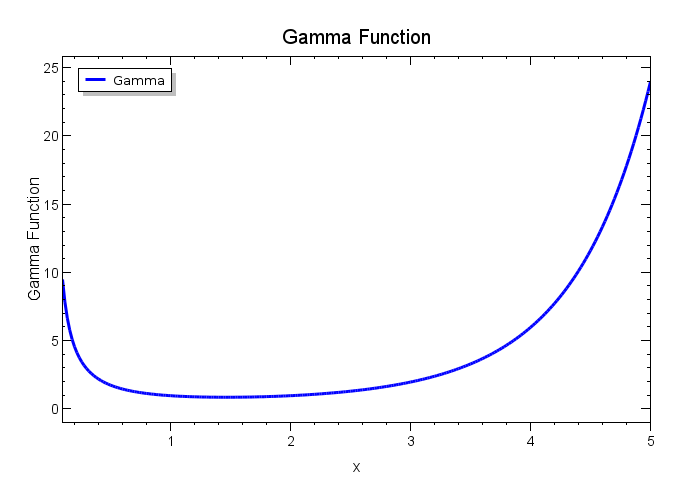
\includegraphics[width=8cm]{gammaFn.png}
   \caption{The gamma function.}
   \label{gammaFig}
\end{figure}

\noindent Procedure \texttt{Beta} returns the beta function 
for its two arguments. The beta function $B (m,n)$ is defined by
\begin{displaymath}
   B (m,n) = \frac{\Gamma (m) \, \Gamma (n)}{\Gamma (m+n)}
\end{displaymath}
which generalizes the product of two factorials.

\noindent Procedure \texttt{MittagLeffler} returns the two-parameter 
Mittag-Leffler function $E_{\alpha , \beta} (x)$ for parameter 
ranges of $0 < \alpha \leq 1$ and $\beta = 0$ or 1.  The Mittag-Leffler 
function is defined by
\begin{displaymath}
   E_{\alpha , \beta} (x) = \sum_0^{\infty} \frac{x^k}
   {\Gamma ( \alpha k + \beta )} 
\end{displaymath}
with graphs for $E_{\alpha , \beta}(x)$ of relevance to the author 
being shown in Fig.~\ref{mittagLefflerFig}.

\begin{figure}
   \centering
   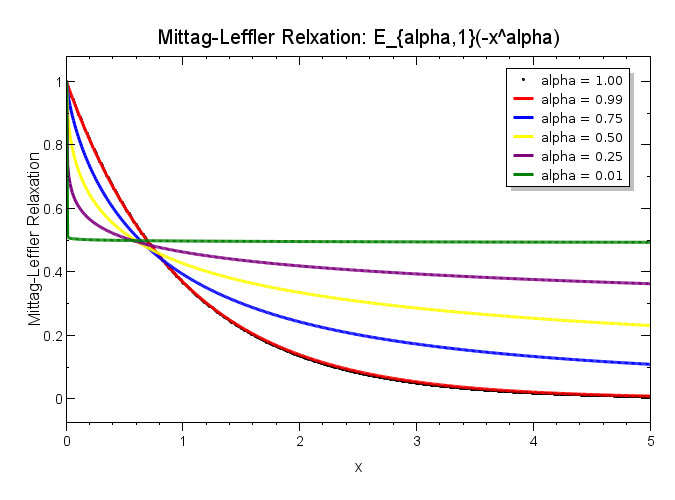
\includegraphics[width=8cm]{mlRelaxFn.png}
   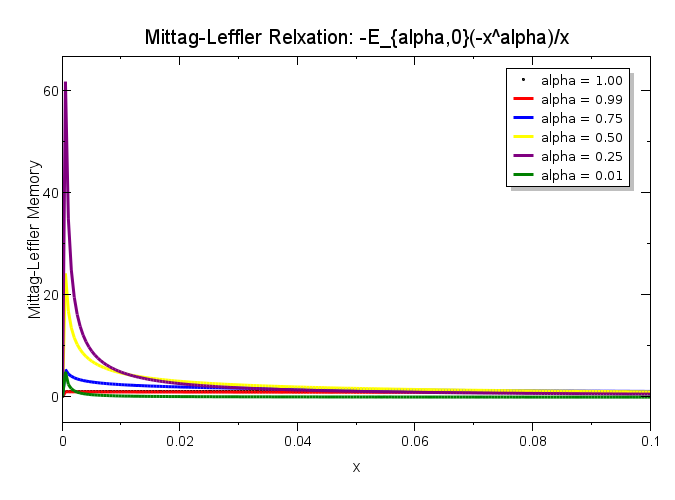
\includegraphics[width=8cm]{mlMemoryFn.png}
   \caption{The Mittag-Leffler function as a relaxation function 
   in viscoelasticity ($E_{\alpha,1}(-x^{\alpha})$) on top, 
   and as a memory function ($-E_{\alpha,0}(-x^{\alpha})/x$) below.}
   \label{mittagLefflerFig}
\end{figure}


\subsection{Interpolations}

Module \texttt{BelMath.Interpolations} provides several functions for
interpolating between data points.

\textsc{Neville}'s algorithm provides an efficient implementation of
\textsc{Lagrange} interpolation.  If vector $\vecMtx{x}$ represents inputs
and vector $\vecMtx{y}$ its outputs, with arrays \texttt{xVec} and \texttt{yVec}
holding their values, then \texttt{Neville} returns the \textsc{Lagrange}
interpolation for value $y$ at some intermediate point $x$ residing within
the range of $\vecMtx{x}$.

A different approach to interpolation is that of \textsc{Hermite}
interpolation.  Procedure \texttt{Hermite} implements a cubic interpolator
where \texttt{xLo} and \texttt{xHi} bound the interval of interpolation
in the independent varibable $x$; \texttt{yLo} and \texttt{yHi} hold
arrays for the dependent variables $\vecMtx{y}$ at these limits, \ie
$\mathtt{yLo} = \vecMtx{y}(\mathtt{xLo})$ and $\mathtt{yHi} =
\vecMtx{y}(\mathtt{xHi})$; and \texttt{dyLo} and \texttt{dyHi} hold the
arrays for the gradient of the dependent variables $\mathrm{d}\vecMtx{y}/
\mathrm{d}x$ at these limits, \ie $\mathtt{dyLo} = \mathrm{d}\vecMtx{y}
(\mathtt{xLo})/\mathrm{d}x$ and $\mathtt{dyHi} = \mathrm{d}\vecMtx{y}
(\mathtt{xHi})/\mathrm{d}x$.  The location for interpolation is sent via
the argument \texttt{x}, with a cubic interpolation being returned by
procedure \texttt{Hermite}, \viz $\vecMtx{y}(\mathtt{x})$.

Two-dimensional interpolation over a rectangular grid is accommodated with
\texttt{Bilinear}.  Supplied values are the $x$ and $y$ grid coordinates,
with \texttt{x1} < \texttt{x2} and \texttt{y1} < \texttt{y2}; their held
values \texttt{valX1Y1, valX1Y2, valX2Y1} and \texttt{valX2Y2}; and the
grid coordinates where the interpolation is sought: \texttt{atX} and
\texttt{atY}, with \texttt{x1} $\leq$ \texttt{atX} $\leq$ \texttt{x2}
and \texttt{y1} $\leq$ \texttt{atY} $\leq$ \texttt{y2}.


\subsection{Distributions}

\texttt{BelMath.Distributions} has, at present, three distributions in it:
the chi-squared distribution, the Student's t-distribution, and the F
distribution.

This module exports an enumerated type, \texttt{Certainty}, that has values:
\texttt{ninety}, \texttt{ninetyFive}, \texttt{ninetySevenPointFive},
\texttt{ninetyNine} and \texttt{ninetyNinePointFive}. For any of these
percentage point certainties, one can get the \texttt{StudentT} or
\texttt{F} distribution values for any degree of freedom, or the
\texttt{ChiSquaredLow} and \texttt{ChiSquaredHigh} distribution values up
through 100 degrees of freedom.

Given that $x_1, x_2, \dots , x_\nu$ are $\nu$, independent, normally
distributed, standardized, random variables (\ie they have a mean of zero,
and a variance of one),
then $X^2 = \sum_{n=1}^\nu x_i^2$ is said to follow a \textit{chi-squared\/}
distribution in $\nu$ degrees of freedom, with the probability that
$X^2 \leq \chi^2$ being given by $P(\chi^2 | \nu)$.  \texttt{ChiSquaredLow}
returns $\chi^2_{\alpha} (\nu)$ and \texttt{ChiSquaredHigh} returns
$\chi^2_{1-\alpha} (\nu)$ for probabilities (or percentage-point
certainties) of $(1-\alpha)100\%$.

Given that $X$ is a normally distributed, standardized, random variable,
and that $\chi^2$ is a random variable following an independent, chi-squared
distribution in $\nu$ degrees of freedom, then the probability 
$P \bigl( \bigl| X / \sqrt{ \chi^2 / \nu} \bigr| \leq t \bigr)$ is
Student~t distributed.  \texttt{StudentT} returns $t_{\alpha} (\nu)$ for
probabilities (or percentage-point certainties) of $(1-\alpha)100\%$.

Given that $X_1^2$ and $X_2^2$ are two, independent, random variables distributed
chi-squared in $\nu_1$ and $\nu_2$ degrees of freedom, respectively, then the
variance ratio $F = ( X_1^2 / \nu_1 ) / ( X_2^2 / \nu_2 )$ is distributed F
with distribution function $P(F | \nu_1 , \nu_2)$.  \texttt{F} returns
$F_{\alpha} (\nu_1,\nu_2)$ for probabilities (or percentage-point certainties)
of $(1-\alpha)100\%$.  The ordering of $\nu_1$ and $\nu_2$ matters.
An important reflexive property of the F-distribution is that
$F_{1-\alpha} (\nu_1, \nu_2) = 1 / F_{\alpha} (\nu_2, \nu_1)$.


\subsection{Random Variates}

\texttt{BelMath.RandomVariates} provide random numbers that are 
distributed according to specified distributions.  Procedure 
\texttt{Normal} returns a random normal variable with a mean of 
zero and a standard deviation of one.  Procedure \texttt{Exponential} 
returns a random exponential variable with a mean and standard 
deviation of one.  They implement the ziggurat method of
Marsaglia \& Tsang \cite{MarsagliaTsang84}.


\subsection{Regression}

Least-squares regression is a technique that can be used to fit some basic
models to experimental data, which is what the routines in module
\texttt{BelMath.Regression} do.  Given a vector of inputs $\vecMtx{x}$
to which there corresponds a vector of outputs $\vecMtx{y}$ of like dimension,
procedure \texttt{Linear} fits these data to the function $\tenMtx{y}_i =
k_0 + k_1 \tenMtx{x}_i$, while procedure \texttt{Quadratic} fits these
same data to the function $\tenMtx{y}_i = k_0 + k_1 \tenMtx{x}_i + k_2
\tenMtx{x}_i^2$, where $k_0$, $k_1$ and $k_2$ are the fit parameters.

It is often useful to map the data into a range where the data can be
fit by a linear or quadratic least-squares process.  Several mappings
to linear fits are provided:  Procedure \texttt{Exponential} fits the
data to function $\tenMtx{y} = k_0 \exp ( k_1 \tenMtx{x} )$,
while procedure \texttt{PowerLaw} fits them to $\tenMtx{y} = k_0
\tenMtx{x}^{k_1}$, and \texttt{StretchedExp} fits them to
$\tenMtx{y} = \exp ( k_0 \tenMtx{x}^{k_1} )$.
The quadratic model can be applied to mapped arguments for $\vecMtx{x}$
and\slash or $\vecMtx{y}$, too, but no precanned procedures are provided
for such models.  The users will have to create such maps for themselves.

All regression procedures return the $R^2$ statistic for goodness of fit,
a.k.a.\ the coefficient of determination.  For the exponential model,
the $R^2$ statistic is calculated in an $x$ \vs $\log y$ plot of the data.
For the power-law model, the $R^2$ statistic is calculated in an $\log x$
\vs $\log y$ plot of the data.  And for the stretched-exponential model,
the $R^2$ statistic is calculated in an $\log x$ \vs $\log ( \log y )$
plot of the data.


\subsection{Roots}
\label{rootsSection}

\texttt{BelMath.Roots} provides algorithms for solving $\vecMtx{f} (
\vecMtx{x}) = \vecMtx{0}$, \viz to find a value for $\vecMtx{x}$ such
that function $\vecMtx{f}$ evaluated at $\vecMtx{x}$ gives zero.  This
module exports two procedure types: \texttt{F} is the type in which the
function $\vecMtx{f}$ is to be supplied and, when needed, \texttt{J} is
the type that its Jacobian, \ie $\mathrm{d} \vecMtx{f} / \mathrm{d}
\vecMtx{x}$, is to be supplied in.

\textsc{Newton}'s method, exported as the procedure \texttt{Newton}, is the
predominant algorithm used to find roots of a function.  Its first argument
is an instance of type \texttt{F}, or the function whose roots are to be found.
The second is of type \texttt{J}, or the function for acquiring the Jacobian
of function \texttt{F}.  The final argument of \texttt{Newton} is the
argument $\vecMtx{x}$ of function $\vecMtx{f}$, whose sent value is an
initial guess at this root, and whose returned value is the actual root.
\textsc{Newton}'s method needs a good initial guess at where a particular 
root may be, otherwise it is likely to become unstable.  Multiple roots 
are common, often residing at different locations $\vecMtx{x}$, so 
choosing an initial guess close to the desired root is an important 
consideration when using \texttt{Newton}.

\textsc{Newton}'s method requires a Jacobian.  If an analytic Jacobian is not
available, for whatever reason, then procedure \texttt{NumericalJacobian}
can be called from within the programmer's implementation of procedure
type \texttt{J} to be used to estimate its value.  In addition to the
interface of procedure type \texttt{J}, \texttt{NumericalJacobian} requires
an instance of type \texttt{F} to be passed as an argument.  This procedure
estimates the Jacobian using a midpoint difference.  Alternatively, 
if the supplied Jacobian for procedure \texttt{Newton} is \texttt{nil} 
then \texttt{NumericalJacobian} is called internally to approximate 
the actual Jacobian.


\section{Calculus}

A variety of numerical methods have been implemented for approximating
the various operators of the calculus; in particular: algorithms for
approximating derivatives, integrals, ordinary differential equations
(ODE), and convolution integrals are provided.


\subsection{Derivatives}

Module \texttt{BelMath.Derivatives} exports the enumerated type
\texttt{Method} from which a programmer can choose one of four methods
for numerically differentiating a user-supplied function.
These four choices are: \texttt{forward}, \texttt{central},
\texttt{backward} and \texttt{richardson}. Procedure
\texttt{Differentiate} estimates $\mathrm{d} y (x) / \mathrm{d} x$.
It has arguments that include the user function to be differentiated
`\texttt{y}' (an instance of exported procedure type \texttt{Y}),
the value of the independent variable where this derivative
is to be estimated `\texttt{x}', the step size that is to be used in the
approximation `\texttt{h}', and the method to be used for approximation
`\texttt{m}'. Only method \texttt{richardson} subdivides the interval to
improve upon accuracy.

Sometimes one knows what step size $h$ to use, but typically one just
wants that step size which when used will enable the most accurate
estimate possible for a given numerical method.  A call to procedure \texttt{OptimalStepSize} returns such an $h$.  This will depend upon the
value of the independent variable $x$ at which the derivative is to
be gotten, which is passed as argument \texttt{atX}.


\subsection{Integrals}

\texttt{BelMath.Integrals} also exports an enumerated type
\texttt{Method} from which the programmer can now choose one of five methods
for numerically integrating a user-supplied function.  The choices
include: \texttt{trapezoidal}, \texttt{simpson}\footnote{%
   \fontsc{Simpson}'s rule, as a method for approximating volumes, can be
   traced back to the works of \textsc{Johannes Kepler}, about one hundred
   years before \textsc{Thomas Simpson} was born.  \textsc{Kepler} used
   this algorithm to estimate the volume of wine casks.},
\texttt{threeEights}, \texttt{romberg} and \texttt{gauss}. Procedure
\texttt{Integrate} estimates $\int_a^b f(x) \; \mathrm{d} x$.  It
has arguments that include the user function to be
integrated `\texttt{f}' (an instance of exported procedure type \texttt{F}),
the lower- and upper-limits of integration `\texttt{a}' and `\texttt{b}',
and the method of approximation `\texttt{m}'. Only methods \texttt{romberg}
and \texttt{gauss} subdivide the interval to improve upon accuracy.


\subsection{Runge-Kutta ODE Solvers}
\label{RKsolvers}

Given some ordinary differential equation (ODE) $\mathrm{d} \vecMtx{y} /
\mathrm{d} x = \vecMtx{f} ( x , \vecMtx{y} )$, a \textsc{Runge}-\textsc{Kutta}
(RK) integrator seeks to acquire an estimate for its solution by getting estimates
$\vecMtx{y}_i = \vecMtx{y}_n + h \sum_{j=1}^s \tenEle{A}_{ij} \vecMtx{F}_j$
at $s$ stage locations $x_i = x_n + \vecEle{c}_i h$ across the interval
$[x_n , x_{n+1}]$.  Specifically, stage derivatives $\vecMtx{F}_i$ are
evaluated at quadrature positions $x_i$ according to the formula
\begin{displaymath}
   \vecMtx{F}_i = \vecMtx{f} \bigl( x_n + \vecEle{c}_i h , \vecMtx{y}_n + h
   \textstyle{\sum_{j=1}^s} \tenEle{A}_{ij} \vecMtx{F}_j \bigr) ,
\end{displaymath}
with its quadrature of integration being given by
\begin{displaymath}
   \vecMtx{y}_{n+1} = \vecMtx{y}_n + h \sum_{i=1}^s \vecEle{b}_i \vecMtx{F}_i .
\end{displaymath}
Specific \textsc{Runge}-\textsc{Kutta} integrators are typically quantified by their
individual \textsc{Butcher} tableau \cite{Butcher08}
\begin{displaymath}
  \begin{tabular}{c|c}
     $\vecFld{c}$ & $\tenFld{A}$ \\ \hline
      & $\vecFld{b}^{T^{\vphantom{|}}}$
  \end{tabular} .
\end{displaymath}
A method will be explicit whenever its $\tenFld{A}$ matrix is lower triangular,
as are the cases addressed below.

At the suggestion of Prof.\ \textsc{John Butcher}, \textsc{Richardson}
extrapolation is employed to arrive at an asymptotically correct estimate
of the local truncation error.  By using the same integrator twice, the
first time advancing a solution $\vecMtx{y}_1$ with a single step size of $h$,
and the second time by advancing a solution $\vecMtx{y}_2$ from two successive
half-steps of size $h/2$, then the truncation error is given by
\begin{displaymath}
   \mathrm{err} = \frac{\| \vecMtx{y}_2 - \vecMtx{y}_1 \|}{1 - 2^{-p}}
   + O (h^{p+2}) ,
\end{displaymath}
where $p$ is the order of the method, \eg \scalar{4} for \fontsc{Kutta}'s
original method.  This error is held to a tolerance specified by 
the user at the time of \texttt{SetUp} by employing \fontsc{S\"oderlind}'s
\cite{Gustafssonetal88,Soderlind02} PI control technology to 
dynamically adjust the step-size for optimum performance.


\begin{table}
 \begin{displaymath} \mbox{}\hspace{2.25cm}
  \begin{array}{l  |  l@{}l@{}}
   \text{\scalar{0}} & \text{\scalar{0}} & \m\text{\scalar{0}} \\
   \text{\scalar{1}} & \text{\scalar{1}} & \m\text{\scalar{0}} \\ \hline
   \vphantom{\tfrac{1}{1}} & \text{\scalar{1}}/\text{\scalar{2 }}
   & \m\text{\scalar{1}}/\text{\scalar{2}}
  \end{array}
 \end{displaymath}
 \caption{Trapezoidal rule.}
 \label{RK2}
\end{table}

\begin{table}
 \begin{displaymath}\mbox{}\hspace{1.5cm}
  \begin{array}{l  |  l@{}l@{}l@{}}
   \text{\scalar{0}} & \m\text{\scalar{0}} & \m\text{\scalar{0}}
      & \m\text{\scalar{0}} \\
   \text{\scalar{1}}/\text{\scalar{2}}  & \m\text{\scalar{1}}/\text{\scalar{2}}
      & \m\text{\scalar{0}} & \m\text{\scalar{0}} \\
   \text{\scalar{1}} & -\text{\scalar{1}}  & \m\text{\scalar{2}}
      & \m\text{\scalar{0}}\\ \hline
   \vphantom{\tfrac{1}{1}} & \m\text{\scalar{1}}/\text{\scalar{6}}
      & \m\text{\scalar{2}}/\text{\scalar{3}}
      & \m\text{\scalar{1}}/\text{\scalar{6}}
  \end{array}
 \end{displaymath}
 \caption{A third-order \mbox{\textsc{Runge-Kutta}} integrator that utilizes
 the weights and quadrature points of \mbox{\textsc{Simpson}}'s rule, a.k.a.\
 \mbox{\textsc{Kepler}}'s cask rule.}
 \label{RK3}
\end{table}


\begin{table}
 \begin{displaymath}\mbox{}\hspace{1cm}
  \begin{array}{l  |  l@{}l@{}l@{}l@{}}
   \text{\scalar{0}}   & \m\text{\scalar{0 }}   & \m\text{\scalar{0 }}
      & \m\text{\scalar{0 }} & \m\text{\scalar{0}} \\
   \text{\scalar{1}}/\text{\scalar{3}} & \m\text{\scalar{1}}/\text{\scalar{3}}
      & \m\text{\scalar{0}} & \m\text{\scalar{0}} & \m\text{\scalar{0}} \\
   \text{\scalar{2}}/\text{\scalar{3}} & -\text{\scalar{1}}/\text{\scalar{3}}
      & \m\text{\scalar{1}} & \m\text{\scalar{0}} & \m\text{\scalar{0}} \\
   \text{\scalar{1}} & \m\text{\scalar{1}}
      & -\text{\scalar{1}} & \m\text{\scalar{1}} & \m\text{\scalar{0}} \\ \hline
   \vphantom{\tfrac{1}{1}} & \m\text{\scalar{1}}/\text{\scalar{8}}
      & \m\text{\scalar{3}}/\text{\scalar{8}}
      & \m\text{\scalar{3}}/\text{\scalar{8}}
      & \m\text{\scalar{1}}/\text{\scalar{8}}
  \end{array}
 \end{displaymath}
 \caption{\mbox{\textsc{Kutta}}'s
   \mbox{\scalar{3}/\scalar{8}}$\mbox{}^{\text{th}}$ rule.
   His most accurate \mbox{\textsc{Runge-Kutta}} method.}
 \label{RK4}
\end{table}

\begin{table}
 \begin{displaymath} \mbox{}\hspace{-0.5cm}
  \begin{array}{l  |  l@{}l@{}l@{}l@{}l@{}l@{}}
   \text{\scalar{0}}   & \m\text{\scalar{0}}   & \m\text{\scalar{0}}
      & \m\text{\scalar{0}} & \m\text{\scalar{0}} & \m\text{\scalar{0}}
      & \m\text{\scalar{0}} \\
   \text{\scalar{1}}/\text{\scalar{4}} & \m\text{\scalar{1}}/\text{\scalar{4}}
      & \m\text{\scalar{0}} & \m\text{\scalar{0}} & \m\text{\scalar{0}}
      & \m\text{\scalar{0}} & \m\text{\scalar{0}} \\
   \text{\scalar{1}}/\text{\scalar{4}} & \m\text{\scalar{1}}/\text{\scalar{8}}
      & \m\text{\scalar{1}}/\text{\scalar{8}}  & \m\text{\scalar{0}}
      & \m\text{\scalar{0}} & \m\text{\scalar{0}} & \m\text{\scalar{0}} \\
   \text{\scalar{1}}/\text{\scalar{2}} & \m\text{\scalar{0}}
      & \m\text{\scalar{0}} & \m\text{\scalar{1}}/\text{\scalar{2}}
      & \m\text{\scalar{0}} & \m\text{\scalar{0}} & \m\text{\scalar{0}} \\
   \text{\scalar{3}}/\text{\scalar{4}} & \m\text{\scalar{3}}/\text{\scalar{16}}
      & -\text{\scalar{3}}/\text{\scalar{8}}
      & \m\text{\scalar{3}}/\text{\scalar{8}}
      & \m\text{\scalar{9}}/\text{\scalar{16}}
      & \m\text{\scalar{0}} & \m\text{\scalar{0}} \\
   \text{\scalar{1}} & -\text{\scalar{3}}/\text{\scalar{7}}
      & \m\text{\scalar{8}}/\text{\scalar{7}}
      & \m\text{\scalar{6}}/\text{\scalar{7}}
      & -\text{\scalar{12}}/\text{\scalar{7}}
      & \m\text{\scalar{8}}/\text{\scalar{7}} & \m\text{\scalar{0}} \\ \hline
   \vphantom{\tfrac{1}{1}}
      & \m\text{\scalar{7}}/\text{\scalar{90}}
      & \m\text{\scalar{0}}
      & \m\text{\scalar{16}}/\text{\scalar{45}}
      & \m\text{\scalar{2}}/\text{\scalar{15}}
      & \m\text{\scalar{16}}/\text{\scalar{45}}
      & \m\text{\scalar{7}}/\text{\scalar{90}}
  \end{array}
 \end{displaymath}
 \caption{A fifth-order \mbox{\textsc{Runge-Kutta}} method derived by
      \mbox{\textsc{Butcher}} \cite[pg.~191]{Butcher08}.}
 \label{RK5}
\end{table}

\begin{table*}
 \begin{displaymath} \mbox{}\hspace{2.25cm}
  \begin{array}{l  |  l@{}l@{}l@{}l@{}l@{}l@{}l@{}}
   \text{\scalar{0}}   & \m\text{\scalar{0}}   & \m\text{\scalar{0}}
      & \m\text{\scalar{0}} & \m\text{\scalar{0}} & \m\text{\scalar{0}}
      & \m\text{\scalar{0}} & \m\text{\scalar{0}} \\
   \text{\scalar{1}}/\text{\scalar{3}} & \m\text{\scalar{1}}/\text{\scalar{3}}
      & \m\text{\scalar{0}} & \m\text{\scalar{0}} & \m\text{\scalar{0}}
      & \m\text{\scalar{0}} & \m\text{\scalar{0}} & \m\text{\scalar{0}} \\
   \text{\scalar{2}}/\text{\scalar{3}} & \m\text{\scalar{0}}
      & \m\text{\scalar{2}}/\text{\scalar{3}} & \m\text{\scalar{0}}
      & \m\text{\scalar{0}} & \m\text{\scalar{0}} & \m\text{\scalar{0}}
      & \m\text{\scalar{0}} \\
   \text{\scalar{1}}/\text{\scalar{3}} & \m\text{\scalar{1}}/\text{\scalar{12}}
      & \m\text{\scalar{1}}/\text{\scalar{3}}
      & -\text{\scalar{1}}/\text{\scalar{12}}
      & \m\text{\scalar{0}} & \m\text{\scalar{0}} & \m\text{\scalar{0}}
      & \m\text{\scalar{0}} \\
   \text{\scalar{5}}/\text{\scalar{6}} & \m\text{\scalar{25}}/\text{\scalar{48}}
      & -\text{\scalar{55}}/\text{\scalar{24}}
      & \m\text{\scalar{35}}/\text{\scalar{48}}
      & \m\text{\scalar{15}}/\text{\scalar{8}}
      & \m\text{\scalar{0}} & \m\text{\scalar{0}} & \m\text{\scalar{0}} \\
   \text{\scalar{1}}/\text{\scalar{6}} & \m\text{\scalar{3}}/\text{\scalar{20}}
      & -\text{\scalar{11}}/\text{\scalar{24}}
      & -\text{\scalar{1}}/\text{\scalar{8}}
      & \m\text{\scalar{1}}/\text{\scalar{2}}
      & \m\text{\scalar{1}}/\text{\scalar{10}}
      & \m\text{\scalar{0}} & \m\text{\scalar{0}} \\
   \text{\scalar{1}} & -\text{\scalar{261}}/\text{\scalar{260}}
      & \m\text{\scalar{33}}/\text{\scalar{13}}
      & \m\text{\scalar{43}}/\text{\scalar{156}}
      & -\text{\scalar{118}}/\text{\scalar{39}}
      & \m\text{\scalar{32}}/\text{\scalar{195}}
      & \m\text{\scalar{80}}/\text{\scalar{39}}
      & \m\text{\scalar{0}} \\ \hline
   \vphantom{\tfrac{1}{1}}
      & \m\text{\scalar{13}}/\text{\scalar{200}}
      & \m\text{\scalar{0}}
      & \m\text{\scalar{11}}/\text{\scalar{40}}
      & \m\text{\scalar{11}}/\text{\scalar{40}}
      & \m\text{\scalar{4}}/\text{\scalar{25}}
      & \m\text{\scalar{4}}/\text{\scalar{25}}
      & \m\text{\scalar{13}}/\text{\scalar{200}}
  \end{array}
 \end{displaymath}
 \caption{A sixth-order \mbox{\textsc{Runge-Kutta}} method derived by
      \mbox{\textsc{Butcher}} \cite[pg.~194]{Butcher08}.}
 \label{RK6}
\end{table*}


Module \texttt{BelMath.RungeKutta} implements five, explicit, 
\textsc{Runge-Kutta} integrators, each with a different order 
of accuracy, chosen by selecting an instance of enumerated 
type \texttt{Order}, which includes options: \texttt{second},
\texttt{third}, \texttt{fourth}, \texttt{fifth} and \texttt{sixth}.  
The second-order method uses the quadrature and weights of 
trapezoidal integration, as specified in Table~\ref{RK2}.
The third-order method employees \fontsc{Simpson}'s quadrature 
and weights, as specified in Table~\ref{RK3}.  The fourth-order 
method is \fontsc{Kutta}'s most accurate integrator \cite{Kutta01}, 
which is based on \fontsc{Simpson}'s $\text{\scalar{3}} / 
\text{\scalar{8}}^{\text{th}}$ rule, and is listed in
Table~\ref{RK4}.  While the fifth- and sixth-order methods of
Tables~\ref{RK5} \& \ref{RK6} were taken from \fontsc{Butcher}'s 
textbook on the subject \cite{Butcher08}.  This module exports 
a \texttt{Bel.Entity} object called \texttt{Integrator} that 
preforms \textsc{Runge-Kutta} integration.

Module \texttt{BelMath.RungeKutta} also exports a procedure type
\texttt{F}.  The user
must cast their system of ordinary differential equations (ODEs)
in terms of this interface.  Method \texttt{SetUp} of
type \texttt{Integrator} is called at the start of a solution at which
time one sends: the ODE to be solved `\texttt{f}' (an instance of
procedure type \texttt{F}), the size of the initial time step `\texttt{h}',
the error tolerance `\texttt{tol}' (usually set to a value of $10^{-p}$
where $p$ is the order of the method), and finishing with `\texttt{ord}'
(the order $p$ of the method).  As a rule-of-thumb, for two
significant figures of accuracy, set \texttt{tol} to \scalar{0.01}
and choose the RK integrator with \texttt{ord} set to \texttt{second}.
For three significant figures of accuracy, set \texttt{tol} to \scalar{0.001}
and choose the RK integrator with \texttt{ord} set to \texttt{third}, \etc

There are three \boldtt{var } arguments in method \texttt{Integrate}.
The first is the independent variable \texttt{x}, the second is an
array holding the dependent variables \texttt{y}, and the last of
these fields provides an asymptotically correct estimate for the local
truncation error, \texttt{err}.  Arguments \texttt{x} and \texttt{y}
are input\slash output variables, while argument \texttt{err} is
strictly an output variable.  A call to this method advances the
solution by a single step, whose magnitude is controlled internally
by a proportional integral (PI) controller 
\cite{Gustafssonetal88,Soderlind02}.

The exported variable \texttt{functionEvaluations} specifies the number
of function evaluations required to obtain a solution, while
\texttt{integrationSteps} keeps track of the number of successfully
completed integration steps.  The solver will automatically restart
itself with a reduced step size whenever an asymptotic error estimate
exceeds the error tolerance specified by the user.  When this happens,
it will increment the \texttt{restarts} counter.  These counters are
reset by \texttt{Initialize} and \texttt{SetUp}.


\subsection{General Linear ODE Solvers}

Inherent \textsc{Runge-Kutta} stable (IRKS) methods are a sub-class to a
larger class of numerical methods known as general linear (GL) methods.
GL methods seek to capture the best attributes from \textsl{multi-stage\/}
\textsc{Runge-Kutta} methods, like those presented in \S\ref{RKsolvers},
and combine these with the best attributes from \textsl{multi-step\/}
\textsc{Adams-Bashforth}\slash \textsc{Moulton} methods.  The mathematics
underlying these methods are sophisticated, even daunting at times, the
details of which can be studied in \textsc{Butcher}'s \cite{Butcher08}
textbook by the interested reader.  Only an overview is presented
herein, sufficient for a programmer to understand how these integrators
work, conceptually, and how one would go about implementing them into code,
if need be.  Two, third-order, IRKS methods taken from the author's 
book \cite[App.~D]{Freed13} are presented here.  IRKS methods that 
range from order two to order six can be found at the website
\small\texttt{www.math.auckland.ac.nz/\textasciitilde hpod/atlas}.
\normalsize
The methods from that website are not self starting.

In GL methods, $r$ quantities $\vecMtx{y}_1^{[n-1]}$, $\vecMtx{y}_2^{[n-1]}$,
$\ldots ,$ $\vecMtx{y}_r^{[n-1]}$, which are the history or multi-step values
acquired over previous integration steps, are updated via integration
from step $n-1$ to step $n$, thereby producing a subsequent set of new values
$\vecMtx{y}_1^{[n]}$, $\vecMtx{y}_2^{[n]}$, $\ldots ,$ $\vecMtx{y}_r^{[n]}$,
each being an array of dimension $N$, the number of simultaneous equations
being solved.  During the multi-stage integration from step $n-1$ to step $n$,
$s$ stage values $\vecMtx{Y}_1$, $\vecMtx{Y}_2$, $\ldots$, $\vecMtx{Y}_s$
are computed over this interval, along with their $s$ stage derivatives
$\vecMtx{F}_1$, $\vecMtx{F}_2$, $\ldots$, $\vecMtx{F}_s$.  These resulting
arrays are assembled into superarrays with \textsc{Nordsieck} scaling,
\ie the values over the past $r$ steps going back into the history are
brought forward to the current step as a truncated \textsc{Taylor} series
expansion of the form
\begin{displaymath}
   \mbf{y}^{[n]} =
      \LEFTRIGHT\lcbrace\rcbrace{ \begin{matrix}
         \vecMtx{y}_1^{[n]} \phantom{|} \\
         \vecMtx{y}_2^{[n]} \phantom{|} \\
         \vecMtx{y}_3^{[n]} \phantom{|} \\
         \vdots \phantom{|} \\
         \vecMtx{y}_r^{[n]} \phantom{|}
      \end{matrix} } =
      \LEFTRIGHT\lcbrace\rcbrace{ \begin{matrix}
         \vecMtx{y} (x_n) \\
         h \vecMtx{y}^{\prime} (x_n) \\
         h^2 \vecMtx{y}^{\prime\prime} (x_n) \\
         \vdots \\
         h^{r-1} \vecMtx{y}^{(r-1)} (x_n)
      \end{matrix} } ,
\end{displaymath}
\begin{displaymath}
   \mbf{Y} = \LEFTRIGHT\lcbrace\rcbrace{
       \begin{matrix}
         \vecMtx{Y}_1 \phantom{|} \\
         \vecMtx{Y}_2 \phantom{|} \\
         \vecMtx{Y}_3  \phantom{|}\\
         \vdots  \phantom{|} \\
         \vecMtx{Y}_s \phantom{|}
      \end{matrix} } , \qquad
   \mbf{F} = \LEFTRIGHT\lcbrace\rcbrace{
      \begin{matrix}
         \vecMtx{F}_1 \phantom{|} \\
         \vecMtx{F}_2 \phantom{|} \\
         \vecMtx{F}_3 \phantom{|} \\
         \vdots \phantom{|} \\
         \vecMtx{F}_s \phantom{|}
      \end{matrix} } ,
\end{displaymath}
where $\vecMtx{y}^{\prime} = \mathrm{d} \vecMtx{y} / \mathrm{d} x$,
\etc, with $\mbf{y}^{[n]}$ being $rN$ in size, and $\mbf{Y}$ and
$\mbf{F}$ both being $sN$ in size, while $h = x_n - x_{n-1}$
is the step size of integration ($x$ being the independent variable of
integration, which is usually time).  For the third-order
IRKS integrators presented in \textsf{BEL}, $r = s = 4$.


\begin{table*}
 \centering
 \begin{displaymath}
  \mbox{}{ \left[
  \begin{array}{@{}l@{}l@{}ll  |  l@{}l@{}l@{}l@{}}
  \m\text{\scalar{0}}        & \m\text{\scalar{0}}         & \m\text{\scalar{0}}        & \text{\scalar{0}}
             & \text{\scalar{1}}           & \m\text{\scalar{0.25}}     & \m\text{\scalar{0.0625}}    & \m\text{\scalar{0.015625}} \\
  \m\text{\scalar{0.845232}} & \m\text{\scalar{0}}         & \m\text{\scalar{0}}        & \text{\scalar{0}}
             & \text{\scalar{1}}           & -\text{\scalar{0.345232}}  & -\text{\scalar{0.172616}}   & -\text{\scalar{0.033481}} \\
  -\text{\scalar{0.0449691}} & \m\text{\scalar{0.882754}}  & \m\text{\scalar{0}}        & \text{\scalar{0}}
             & \text{\scalar{1}}           & -\text{\scalar{0.087785}}  & -\text{\scalar{0.29777}} & -\text{\scalar{0.231759}} \\
  \m\text{\scalar{1.03061}}  & \m\text{\scalar{0.483638}}  & \m\text{\scalar{0.157846}} & \text{\scalar{0}}
             & \text{\scalar{1}}           & -\text{\scalar{0.672094}}  & -\text{\scalar{0.235712}} & \m\text{\scalar{0.177668}} \\
  \hline
  \m\text{\scalar{1.03061}}  & \m\text{\scalar{0.483638}}  & \m\text{\scalar{0.157846}} & \text{\scalar{0}}
             & \text{\scalar{1}}           & -\text{\scalar{0.672094}}  & -\text{\scalar{0.235712}}   & \m\text{\scalar{0.177668}} \\
  \m\text{\scalar{0}}        & \m\text{\scalar{0}}         & \m\text{\scalar{0}}        & \text{\scalar{1}}
             & \text{\scalar{0}}           & \m\text{\scalar{0}}        & \m\text{\scalar{0}}         & \m\text{\scalar{0}} \\
  -\text{\scalar{0.712022}}  & -\text{\scalar{0.63459}}    & -\text{\scalar{0.0665772}} & \text{\scalar{1.06962}}
             & \text{\scalar{0}}           & \m\text{\scalar{0.343573}} & -\text{\scalar{0.0487644}}  & \m\text{\scalar{0.512949}} \\
  -\text{\scalar{0.707945}}  & -\text{\scalar{0.57053}}    & -\text{\scalar{0.210071}}  & \text{\scalar{0.622123}}
             & \text{\scalar{0}}           & \m\text{\scalar{0.866424}} & -\text{\scalar{0.00463586}} & \m\text{\scalar{0.0487644}}
  \end{array}
  \right] }
 \end{displaymath}
 \caption{Partitioned matrix for
     an explicit IRKS method of third order with property F,
     where $\vecMtx{c} = \{ \textfrac{1}{4} , \textfrac{1}{2}
     , \textfrac{3}{4} , 1 \}^T$, with error-estimation coefficients of
     $\phi_0 =$ \scalar{98.267807} and $\grkMtx{\phi} = \{$\scalar{329.071228},
     -\scalar{397.606843}, \scalar{201.071228}, -\scalar{34.267807}$\}^T$
     \cite{Freed13}.
     \normalsize}
 \label{ButcherExplicitIRKS}
\end{table*}

\begin{table*}
 \centering
 \begin{displaymath}
  \mbox{}{ \left[
  \begin{array}{@{}l@{}l@{}ll  |  l@{}l@{}l@{}l@{}}
  \m\text{\scalar{0.225}}    & \m\text{\scalar{0}}         & \m\text{\scalar{0}}        & \text{\scalar{0}}
             & \text{\scalar{1}}           & \m\text{\scalar{0.25}}     & -\text{\scalar{0.05}}       & -\text{\scalar{0.0265625}} \\
  \m\text{\scalar{0.211287}} & \m\text{\scalar{0.225}}     & \m\text{\scalar{0}}        & \text{\scalar{0}}
             & \text{\scalar{1}}      & \m\text{\scalar{0.063713}}      & -\text{\scalar{0.0806435}}  & -\text{\scalar{0.0833663}} \\
  \m\text{\scalar{0.946338}} & -\text{\scalar{0.342943}}   & \m\text{\scalar{0.225}}    & \text{\scalar{0}}
             & \text{\scalar{1}}      & -\text{\scalar{0.0783954}}      & \m\text{\scalar{0.0947737}} &\m\text{\scalar{0.121956}} \\
  \m\text{\scalar{0.52149}}  & -\text{\scalar{0.662474}}   & \m\text{\scalar{0.490476}} & \text{\scalar{0.225}}
             & \text{\scalar{1}}      & \m\text{\scalar{0.425507}}      & \m\text{\scalar{0.216014}}  & -\text{\scalar{0.103603}} \\
  \hline
  \m\text{\scalar{0.52149}}  & -\text{\scalar{0.662474}}   & \m\text{\scalar{0.490476}} & \text{\scalar{0.225}}
             & \text{\scalar{1}}           & \m\text{\scalar{0.425507}} & \m\text{\scalar{0.216014}}  & -\text{\scalar{0.103603}} \\
  \m\text{\scalar{0}}        & \m\text{\scalar{0}}         & \m\text{\scalar{0}} & \text{\scalar{1}}
             & \text{\scalar{0}}           & \m\text{\scalar{0}}        & \m\text{\scalar{0}}         & \m\text{\scalar{0}} \\
  -\text{\scalar{0.0423385}} & \m\text{\scalar{0.695379}}  & -\text{\scalar{0.784079}}  & \text{\scalar{1.0116}}
             & \text{\scalar{0}}           & -\text{\scalar{0.880558}}  & -\text{\scalar{0.521284}}   & \m\text{\scalar{0.774748}} \\      
 \m\text{\scalar{0.077564}} & \m\text{\scalar{0.246379}}  & -\text{\scalar{0.321806}}  & \text{\scalar{0.274145}}
             & \text{\scalar{0}}           & -\text{\scalar{0.276282}}  & -\text{\scalar{0.350743}}   & \m\text{\scalar{0.521284}}
  \end{array}
  \right] }
 \end{displaymath}
 \caption{The partitioned matrix for an L-stable, implicit,
     IRKS method of third order that possesses property F,
     where $\vecMtx{c} = \bigl\{ \textfrac{1}{4} , \textfrac{1}{2}
     , \textfrac{3}{4} , 1 \bigr\}^T$, and whose coefficients for error
     estimation are $\phi_0 =$ \scalar{43.700369} and $\grkMtx{\phi} =
     \{$\scalar{110.801474}, -\scalar{70.202212}, -\scalar{17.198526},
     \scalar{20.299631}$\}^T$ \cite{Freed13}.
     \normalsize}
 \label{ButcherImplicitIRKS}
\end{table*}

GL methods are comprised of four matrices, \viz
$\tenFld{A} = [ \tenEle{A}_{ij} ]_{s \times s}$,
$\tenFld{U} = [ \tenEle{U}_{ij} ]_{s \times r}$,
$\tenFld{B} = [ \tenEle{B}_{ij} ]_{r \times s}$ and
$\tenFld{V} = [ \tenEle{V}_{ij} ]_{r \times r}$,
that appear in a special linear system of equations
used to update the state; specifically,
\begin{multline*}
   \vecMtx{Y}_i = h \sum_{k=1}^s \tenEle{A}_{ik} \vecMtx{F}_k 
   ( \vecMtx{Y}_k ) +
      \sum_{k=1}^r \tenEle{U}_{ik} \vecMtx{y}_k^{[n-1]} , \\
      i = 1, 2, \dots , s ,
\end{multline*}
and
\begin{multline*}
   \vecMtx{y}_i^{[n]} = h \sum_{k=1}^s \tenEle{B}_{ik} \vecMtx{F}_k 
   ( \vecMtx{Y}_k ) +
      \sum_{k=1}^r \tenEle{V}_{ik} \vecMtx{y}_k^{[n-1]} , \\
      i = 1, 2, \dots , r ,
\end{multline*}
where matrix $\tenFld{A}$ contains stage coefficients, akin to a
\textsc{Runge}-\textsc{Kutta} method; matrix $\tenFld{B}$ contains
step coefficients, akin to \textsc{Adams-Bashforth}\slash \textsc{Moulton}
methods; while matrices $\tenFld{U}$ and $\tenFld{V}$ couple these
processes together into a single integration algorithm.

The stage derivatives $\vecMtx{F}_k ( x + c_k h, \{ \vecMtx{Y}_i \} )$,
with $i, k = 1, 2, \dots , s$, depend upon the set of stage values
$\{ \vecMtx{Y}_i \}$.  These derivatives are computed at quadrature points
$c_k$ along the interval of integration $[x,x+h] \equiv [x_{n-1},x_n]$.
The sum on index $k$ over the \textsc{Runge-Kutta}--like $\tenEle{A}_{ik}$
coefficients terminates at $i-1$ for explicit methods, at $i$ for
diagonally implicit methods (like the methods presented below),
or at $s$ for fully implicit
methods, which are neither discussed nor implemented herein.


\subsubsection{Estimate Error}

The \textsc{Butcher} matrix for a GL method is a partitioned
$(s+r) \times (s+r)$ matrix of the form
\begin{equation*}
  \left[ \begin{tabular}{c|c}
     $\tenFld{A}$ & $\tenFld{U}$ \\ \hline
     $\tenFld{B}$ & $\tenFld{V}^{\vphantom{l^l}}$
  \end{tabular} \right] .
\end{equation*}
Property F, a.k.a.\ a first-same-as-last method in the RK
literature, is a desirable property for an IRKS method to have in that
it enables one to compute an asymptotically accurate estimate for the
local truncation error.  It is readily apperent by looking at a method's
\textsc{Butcher} matrix if it can or cannot possess this property.
If it can, then the last row in the $[ \tenFld{A} | \tenFld{U} ]$ matrix will be
identical to the first row in the $[ \tenFld{B} | \tenFld{V} ]$ matrix,
and the second row in the $[ \tenFld{B} | \tenFld{V} ]$ matrix will be all zeros,
except for the last column in matrix $\tenFld{B}$ where there will be a one.

To obtain an estimate of solution error for an IRKS method, 
one first constructs the difference vector
\begin{equation*}
    \grkMtx{\Delta}^{[n]} = h \left( 
    \phi_0 \vecMtx{y}^{\prime [n-1]} - 
    \sum_{i=1}^s \phi_i \vecMtx{F}_i \right) ,
\end{equation*}
from which one can then compute a normalized estimate for the error via
\begin{equation*}
   \mathrm{error}_n = \frac{\| \grkMtx{\Delta}^{[n]} \|}
   {\mathrm{max} \bigl( 1 , \bigl\| \vecMtx{y}^{[n-1]} \bigr\| \bigr)} ,
\end{equation*}
where $\phi_0$ and $\grkMtx{\phi} = \{ \phi_1 , \phi_2 , \dots ,
\phi_s \}^T$ are parameters of the integrator.  Note that $\vecMtx{y}^{[n-1]}$
and $h \vecMtx{y}^{\prime [n-1]}$ are stored as the first two subarrays
in the super\-array $\mbf{y}^{[n-1]}$.


\subsubsection{Step-Size Control}

The PI controller of \fontsc{S\"oderlind } 
\cite{Soderlind02,Gustafssonetal88} 
has been adopted to automatically control the step-size $h$ in an 
optimal manner, maintaining a local truncation error of 0.0001. 
Specifically, if $\epsilon_n < 1.2 \, \epsilon_{\max}$ then
\begin{equation*}
   \frac{h_{n+1}}{h_n} = \begin{cases}
      \left( \frac{\epsilon_{\max}}{\epsilon_n} \right)^{0.15} 
      \left( \frac{\epsilon_{n-1}}{\epsilon_{\max}} \right)^{0.1} & 
      \text{if} \;\; \epsilon_{n-1} < \frac{6}{5} \epsilon_{\max} , \\
      \left( \frac{\epsilon_{\max}}{\epsilon_n} \right)^{0.25} & 
      \text{otherwise,}
   \end{cases}
\end{equation*}
with $\epsilon_{\max}$ set at 0.0001.
If $\epsilon_n > 1.2 \, \epsilon_{\max}$ then
\begin{equation*}
   h_n = h_n
   \left( \frac{\epsilon_{\max}}{\epsilon_n} \right)^{0.33} 
\end{equation*}
and the integration over the step is redone until an acceptable 
error is obtained.  To avoid oscillatory behavior, step-size 
resizing is restricted so that $0.1 \leq h_{n+1} / h_n \leq 5$, 
i.e., anti windup.

Before the step-size $h$ can be controlled, it is necessary to
obtain a reasonable estimate for the initial step-size, viz., $h_0$.  
The software does this by first computing
\begin{displaymath}
   h_0 = \frac{\| \vecMtx{y}_0 \|}{\| \vecMtx{f}(x_0,\vecMtx{y}_0) \|}
   \quad \text{so} \quad
   \epsilon_m \leq h_0 \leq 0.001 
\end{displaymath}
where machine epsilon $\epsilon_m$ is taken to be a lower bound on 
step-size and 0.001 an upper bound.  A forward Euler integration 
then gives an estimate for $\vecMtx{y}_1 = \vecMtx{y}_0 + h_0 \, 
\vecMtx{f}_0$ associated with $\vecMtx{f}_0 = \vecMtx{f}(x_0,\vecMtx{y}_0)$. 
This allows one to estimate $\vecMtx{f}_1 = \vecMtx{f}(x_1,\vecMtx{y}_1)$
wherein $x_1 = x_0 + h_0$.  Trapezoidal integration improves 
the estimate for $\vecMtx{y}_1 = \vecMtx{y}_0 + \frac{1}{2} h_0 
( \vecMtx{f}_0 + \vecMtx{f}_1 )$ that, in turn, allows the 
rates to be improved upon by recalculating function $\vecMtx{f}_1 =
\vecMtx{f}(x_1, \vecMtx{y}_1)$, thereby supplying an improved 
trapezoidal estimate for $\vecMtx{y}_1$.  With these fields in hand, 
one can acquire a reasonable estimate for the initial step-size via
\begin{displaymath}
   h_0 = 2 \left| \frac{\| \vecMtx{y}_0 \| - \| \vecMtx{y}_1 \|}
   {\| \vecMtx{f}_0 \| + \| \vecMtx{f}_1 \|} \right| 
\end{displaymath}
so constrained as to lie within $\epsilon_m \leq h_0 \leq 0.001$. 
This comes from the second-order approximation $\| \vecMtx{y}_1 \|
\approx \| \vecMtx{y}_0 \| + h \| \vecMtx{f}_0 \| + \tfrac{1}{2} h^2 
\| \vecMtx{f}_0^{\prime} \|$ where $\| \vecMtx{f}_0^{\prime} \| \approx 
( \| \vecMtx{f}_1 \| - \| \vecMtx{f}_0 \| ) / h$.  A factor of safety 
is imposed in that $h_0 / 10$ is actually used for the first step, 
from which the step-size controller quickly recovers.  This helps to 
ensure that a reasonable first step-size is adopted, as there is no 
ability to establish an error estimate over this step using the startup 
integrator of Table~\ref{ButcherStarter}.  Whatever error one 
starts with carries through the solution.


\subsubsection{IRKS Methods}

Tables \ref{ButcherExplicitIRKS} \& \ref{ButcherImplicitIRKS} provide
the coefficients for explicit and implicit IRKS methods with property~F
that have been implemented into software.  These two methods are not 
self-starting, so a startup method must be called upon to take the 
first step of integration.  An admissible startup
method for the integrators in Tables \ref{ButcherExplicitIRKS} \&
\ref{ButcherImplicitIRKS} is the integrator listed in
Table~\ref{ButcherStarter}.

\begin{table}
 \centering
 \begin{displaymath}
  \mbox{}\left[
  \begin{tabular}{c|c}
   $\begin{matrix}
     \tfrac{1^{\vphantom{!}}}{4_{\vphantom{j}}} & 0 & 0 & 0 \\
     \tfrac{1}{4} & \tfrac{1^{\vphantom{!}}}{4_{\vphantom{j}}} & 0 & 0 \\
     -\tfrac{5}{4} & \tfrac{7}{4} &
        \tfrac{1^{\vphantom{!}}}{4_{\vphantom{j}}} & 0 \\
     \tfrac{5}{12} & \tfrac{5}{12} & -\tfrac{1}{12} &
        \tfrac{1^{\vphantom{!}}}{4_{\vphantom{j}}}
   \end{matrix}$ &
   $\begin{matrix}
      1 \vphantom{\tfrac{1^!}{1_j}} & 0 & 0 & 0 \\
      1 \vphantom{\tfrac{1^!}{1_j}} & 0 & 0 & 0 \\
      1 \vphantom{\tfrac{1^!}{1_j}} & 0 & 0 & 0 \\
      1 \vphantom{\tfrac{1^!}{1_j}} & 0 & 0 & 0
   \end{matrix}$ \\ \hline
   $\begin{matrix}
     \tfrac{5}{12} & \tfrac{5}{12} & -\tfrac{1}{12} &
        \tfrac{1^{\vphantom{!}}}{4_{\vphantom{j}}} \\
      0 & 0 & 0 & 1^{\vphantom{!}}_{\vphantom{j}} \\
      \tfrac{29}{10} & -\tfrac{67}{10} & \tfrac{7}{10} &
         \tfrac{31^{\vphantom{!}}}{10_{\vphantom{j}}} \\
      \tfrac{56}{5} & -\tfrac{88}{5} & \tfrac{8}{5} &
         \tfrac{24^{\vphantom{!}}}{5_{\vphantom{j}}}
   \end{matrix}$ &
   $\begin{matrix}
      1 \vphantom{\tfrac{1^!}{1_j}} & 0 & 0 & 0 \\
      0^{\vphantom{!}}_{\vphantom{j}} & 0 & 0 & 0 \\
      0 \vphantom{\tfrac{1^!}{1_j}} & 0 & 0 & 0 \\
      0 \vphantom{\tfrac{1^!}{1_j}} & 0 & 0 & 0
   \end{matrix}$
  \end{tabular}
 \right]
 \end{displaymath}
 \caption{Partitioned matrix for
     a viable startup method for the IRKS methods given in Tables
     \protect{\ref{ButcherExplicitIRKS}} \& \protect{\ref{ButcherImplicitIRKS}},
     where $\vecMtx{c} = \bigl\{$\textfrac{1}{4}, \textfrac{1}{2},
     \textfrac{3}{4}, 1$\bigr\}^T$. Created for this author 
     \cite{Freed13} by Prof.\ \mbox{\textsc{John Butcher}}.}
 \label{ButcherStarter}
\end{table}

Explicit integrators, like the one in Table \ref{ButcherExplicitIRKS},
are applicable for non-stiff problems, while implicit integrators, like
the one in Table \ref{ButcherImplicitIRKS}, are required whenever a system
of ODEs exhibits stiffness, as they often do.  To implement an implicit
integrator requires the use of \textsc{Newton}'s method for finding roots,
thereby making these methods more expensive at run time.  Nevertheless,
if a system of ODEs is found to be stiff, then their integration with an
implicit method will be less costly than trying to solve it, forcibly,
with an explicit method, because the step size required by an explicit
method needed to maintain an accurate output in the presence of
stiffness can become extremely small. Oftentimes stability cannot be
achieved under these conditions.


\subsubsection{Software}

Module \texttt{BelMath.Irks} implements the explicit and implicit IRKS
methods just discussed, both of which are thrid-order accurate. 
Unlike the \textsc{Runge-Kutta}
integrator of module \texttt{RungeKutta}, which is a \fontttsl{value\/}\
object, here instances of \texttt{Explicit} and \texttt{Implicit} are
\fontttsl{ref\/}\ objects, and therefore must be created with the
\boldtt{new}\ command.

Two procedure types are exported from this module.
An instance of procedure type \texttt{F} provides the ODE that is to be
integrated, \ie $\vecMtx{f} ( x , \vecMtx{y} ) = \mathrm{d}\vecMtx{y} /
\mathrm{d} x$.  An instance of procedure type \texttt{J} provides its
Jacobian, \viz $\tenMtx{J} ( x , \vecMtx{y} ) = \partial \vecMtx{f}
( x , \vecMtx{y} ) / \partial \vecMtx{y}$. The first argument of both
\texttt{F} and \texttt{J} is a \boldttsl{real},
while their second argument is an \boldtt{array } \texttt{$\{$math$\}$}
\boldtt{* of } \boldttsl{real}.  If an analytic Jacobian is not available,
one can construct a numerical approximation for it by writing a
wrapper around \texttt{NumericalJacobian}, which is a procedure
exported from module \texttt{BelMath.Roots}.

Two integrators are supplied.  Type \texttt{Explicit} provides an explicit
method, while type \texttt{Implicit} provides an implicit method.  They
both export counters \texttt{functionEvaluations}, 
\texttt{integrationFalseStarts}, \texttt{integrationRestarts} and
\texttt{integrationSteps}, with the \texttt{Implicit} integrator also
providing a counter for \texttt{jacobianEvaluations}.  Also exported 
as a read-only value is the independent variable \texttt{x}. 
These types have common type-bound procedures, with a slight 
difference occurring in method \texttt{Start}, where the ODE 
to be solved is passed as variable \texttt{f} of type \texttt{F} 
and, in the case of the implicit integrator, its Jacobian is also 
passed as variable \texttt{j} of type \texttt{J}.
The other arguments of procedure \texttt{Start} include:
the initial value \texttt{x0} for the independent variable $x_0$, 
and the initial value \texttt{y0} for the dependent variable 
$\vecMtx{y}_0$, \ie the initial condition.  Returned is the 
optimal step-size \texttt{h} for the next integration step.

Wherever the system of ODEs is discontinuous, i.e., at any $x$ 
where $\vecMtx{f} ( x_- , \vecMtx{y} ) \neq \vecMtx{y} 
( x_+ , \vecMtx{y} )$, the integrator must be restarted at $x$.  
This is done by calling procedure \texttt{Restart} which returns 
the optimal step-size $h$ for the ensuing integration step.

Integration is normally carried out by procedure \texttt{Integrate} 
where the step-size is both an input and output variable.  The 
user can adjust $h$ for the next integration step, say to hit 
a target value of $x$.  Normally, it is left alone and returned 
in the next call to \texttt{Integrate}.  

The final procedure that is in common with the \texttt{Explicit} 
and \texttt{Implicit} integrators is method \texttt{GetSolution} 
that uses the embedded \textsc{Taylor} series in the 
\textsc{Nordsieck} scaling, thereby insuring a third-order 
accurate estimate to the solution over the entire range of 
integration.  The first argument \texttt{atX} specifies where 
the solution is sought.  The second argument \texttt{y} 
returns this solution, with the final argument specifying the 
local truncation error pertaining to the interval from which 
the solution was extracted.  Module \texttt{BelMath.Irks} 
uses a \texttt{Bel.List} to manage this data base.


\subsection{Convolution Integrals}

Consider a convolution integral of the form
\begin{displaymath}
   \int_0^x \kappa (x - y) \: \vecMtx{f} (y, x) \:
   \mathrm{d} y, \quad x \in [0,X],
\end{displaymath}
where the kernel $\kappa$ and forcing $\vecMtx{f}$ functions are known.
The kernel is a real valued function, while the forcing function is
taken to be an array.  The K-BKZ visco\-elastic models discussed in
the author's book \textit{Soft Solids\/} are described by \textsc{Volterra}
integral equations that contain such convolution integrals.

The algorithm implemented by type \texttt{Integral} in the module
\texttt{BelMath.ConvolutionIntegrals} provides a numerical approximation
for this convolution integral based upon Algorithms 3--6 from
\textsc{Diethelm} \& \textsc{Freed} \cite{DiFreed:conv-quad}, 
and has been republished as App.~E in the author's book \cite{Freed13}.
The interested reader is referred to \cite{DiFreed:conv-quad} 
for substantive details.\footnote{
   There is a typo at the end of Alg.~4 in \cite{DiFreed:conv-quad}.
   It reads: \\
   \mbox{\hspace{1cm}\texttt{FOR i $\coloneq$ 1 TO L$_{\mathrm{n}}$ DO}} \\
   \mbox{\hspace{1cm}\texttt{\mbox{}\phantom{FOR }I $\coloneq$ I + P$_{\mathrm{n}}$[i].}} \\
   It should read: \\
   \mbox{\hspace{1cm}\texttt{FOR i $\coloneq$ 1 TO L$_{\mathrm{n-1}}$ DO}} \\
   \mbox{\hspace{1cm}\texttt{\phantom{FOR }I $\coloneq$ I + P$_{\mathrm{n-1}}$[i].}} \\ 
   This is corrected in \cite[App.~E]{Freed13}.
}

The \textsc{Diethelm}-\textsc{Freed} integrator is more than just
formul\ae; it is a collection of four algorithms.  The first algorithm
manages assignment of an evolving set of quadrature nodes defined
over a  changing interval of integration.  The second algorithm
manages the history variables, keeping them in conformation with
the nodes of quadrature.  The third algorithm handles calls made
to the kernel function.  While the forth algorithm performs a numerical
approximation of this convolution integral using a \textsc{Laplace}
quadrature scheme with end-point correction, resulting in a method
that is fifth-order accurate.  This quadrature scheme allows the kernel
function to be weakly singular, \viz $\kappa(0) = \infty$ is permitted.

For K-BKZ viscoelastic models, the forcing function $\mathbscr{E}$
(strain) is a function of another function $\tenFld{F}$  (the deformation
gradient) that in turn depends on the independent variable of integration,
which is time $t$ in this case, and as such, can be rewritten as $\mathbscr{E}
(t^{\prime},t) = \what{\mathbscr{E}} ( \tenFld{F}(0,t^{\prime}),
\tenFld{F} (0,t))$, or more simply, $\mathbscr{E} (t^{\prime},t) =
\what{\mathbscr{E}} ( \tenFld{F} (t^{\prime}), \tenFld{F}(t))$, where
$\tenFld{F} (t^{\prime})$ implies $\tenFld{F} (0, t^{\prime})$, \etc
When expressed in the format of the above convolution integral,
K-BKZ models look like
\begin{displaymath}
   \int_0^t \kappa (t - t^{\prime}) \, \vecMtx{f} \bigl(
   \vecMtx{g} (t^{\prime}) , \vecMtx{g} (t) \bigr) \, \mathrm{d} t^{\prime},
   \quad t \in [0,T] ,
\end{displaymath}
where the forcing function $\vecMtx{f}$ now depends upon a subordinate function
$\vecMtx{g}$ that is evaluated at two states, \viz $t^{\prime}$ and $t$.  What
this integrator stores in terms of history variables is $\vecMtx{g} (t_j)$,
not $\vecMtx{f} (t_i,t_j)$, where $i \leq j$, which can be done much
more economically.  The algorithm is structured so that as one moves further
along the solution path one can delete some of the earlier $\vecMtx{g} (t_i)$,
since all future samplings will only occur at points other than $t_i$.
Actually, this was a fundamental design criterion for the algorithm
developed in \cite{DiFreed:conv-quad}.  In the more general setting of
the first expression given for the convolution integral, one has
\begin{displaymath}
   \vecMtx{f} (y, x) = \vecMtx{f} \bigl( \vecMtx{g}(y),
   \vecMtx{g}(x) \bigr) ,
\end{displaymath}
where the expression on the right is how the forcing function is
implemented in \textsf{BEL}.

This numerical integrator is built upon three premises. The first is that
some characteristic time $\tau > 0$ quantifies the decay behavior of
kernel $\kappa$.  This parameter is chosen at the beginning of the
process, and is kept fixed throughout the integration.  For visco\-elastic
models, one would likely assign $\tau$ as being the model's characteristic
relaxation time.

The second premise resides with the user selecting the number of
integration steps that are to be applied over the time interval $[0,\tau]$.
This value is assigned to variable $H>4$, with the step-size of integration
$h$ then being set at $h = \tau / H$, where $h$ remains fixed over the
entire interval of integration $[0,T]$.  $H$ must be greater than $4$
because of the quadrature rule selected for integration.

The third premise is the existence of a quality parameter in the form
of an odd cardinal number $Q \in \{ 3, 5, 7, 9, \dots \}$ that is also kept
fixed throughout the process.  A small value for $Q$ will lead to a
fast but not so accurate implementation of the algorithm, while
large choices for $Q$ improve the accuracy, but run slower.

What $Q$ controls is the maximum size of each sub\-interval of integration.
Each sub\-interval can contain $H$, $2H$, $\dots$, or $QH$ nodes, with the
sub\-interval closest to the upper limit containing a possible
$1$ to $H-1$ extra nodes, as deemed necessary
to span the interval of integration $[0,T]$. The step size is fixed over
each sub\-interval, but increases with a logarithmic gait from one
sub\-interval to the next.  Bearing in mind that the kernel $\kappa$
monotonically decays, this suggests the use of a step size of $h$ on the
first sub\-interval, a step size of $Q h$ on the second sub\-interval,
a step size of $Q^2 h$ on the third sub\-interval, \etc
This logarithmic memory concept was introduced by \textsc{Ford} \&
\textsc{Simpson}~\cite{FordSi:speed-acc}.

It is the garbage collector devised by \textsc{Diethelm} in
\cite{DiFreed:conv-quad} for managing the history variables that, when
used in accordance with a \textsc{Ford}-\textsc{Simpson} logarithmic
gait between quadrature nodes, requires the step size of integration
$h$ to be uniform over the whole of the interval of integration $[0,T]$.

\subsubsection{Software}

Module \texttt{BelMath.ConvolutionIntegrals} exports two procedure types.
Instances of \texttt{Kernel} are to describe $\kappa(x - y)$,
while instances of \texttt{ForcingFn} are to describe $\vecMtx{f}(
\vecMtx{g}(y) , \vecMtx{g}(x))$.  Type \texttt{Integral}
exports three numbers: the next integration step will have count
\fonttt{n}, the total number of integration steps required is
stored in \fonttt{N}, while \texttt{xN} designates the value of
the dependent variable $x$ at the end of the next step \fonttt{n}.

Method \texttt{SetUp} contains seven arguments.  The first two arguments,
\texttt{qualityPara} and \texttt{stepsPerCharTime}, are integers that hold
the values for: quality parameter $Q$, and the number of integration
steps $H$ to be used to traverse an interval of width $T$.  The third
and fourth arguments are \boldttsl{real\/}s.
\texttt{xMax} is the upper limit of integration
$X$ at the final step of integration, while \texttt{charTime} is the
characteristic time $T$ associated with the specified kernel.  The fifth argument,
\texttt{gAt0}, is where one passes the initial value for the
subordinate forcing function, \viz $\vecMtx{g}(0)$, to the integrator,
which is an \boldtt{array } \texttt{$\{$math$\}$ } \boldtt{* of }
\boldttsl{real}.
The last two arguments contain instances of types \texttt{Kernel} and
\texttt{ForcingFn}, denoted as \texttt{kernelFn} and \texttt{forcingFn}.

Method \texttt{Integrate} performs the necessary integration to advance a
solution from step $n-1$ to step $n$.  The user supplies $\vecMtx{g}(x_n)$
as argument \texttt{gAtN}, which is the second argument of $\vecMtx{f}$
over the integration, with the first arguments coming from the memory
manager of the integrator.  \texttt{Integrate} returns the value of
the convolution integral whose upper limit is $x_n$.  \texttt{N}
successive calls to this procedure are needed to solve a convolution
integral over some range $[0,X]$.



\section{History of Changes}
\fontsize{10pt}{12pt}\selectfont

\textsf{BEL} version releases wherein no change took place
in \textsf{BelMath} are omitted.  Version numbering corresponds 
with the version releases of \textsf{BEL}.


\subsection{Changes to Version 4.2}

An automatic time-step controller was added to the IRKS integrators.
This required introducing a data base for managing the history of 
integration, which necessitated some changes in the interface, too.


\subsection{Changes to Version 4.1}

Exception handler added to \texttt{BelMath.Roots.Newton} in an effort 
to make it more robust.  The module \texttt{BelMath.SpecialFunctions} 
was created, moving \texttt{Erf}, \texttt{Erfc}, \texttt{Gamma}, 
and \texttt{Beta} from \texttt{Bel.Math} and adding to it the function 
\texttt{MittagLeffler}.


\subsection{Changes to Version 4.0}

Modules \texttt{BelMath.Series} and \texttt{BelMath.Functions} were moved
to the core library as modules \texttt{Bel.Series} and \texttt{Bel.Math},
respectively.  Module \texttt{BelMath.LinearAlgebra} has been depreciated
because of the ability to solve linear systems of equations directly with
calls like \texttt{x := A$\backslash$b}, which solves $\tenMtx{A}
\vecMtx{x} = \vecMtx{b}$ for vector $\vecMtx{x}$ by using the
\textsl{$\{$math$\}$\/} extension for arrays.

All of the modules in this library, including their interfaces,
were altered such that numeric types \texttt{BelTypes.Numbers.Number},
\texttt{BelTypes.Arrays.Array} and \texttt{BelTypes.Matrices.Matrix} were
changed to \boldttsl{real}, \boldtt{array} \texttt{$\{$math$\}$} \boldtt{* of}
\boldttsl{ real } and \boldtt{array} \texttt{$\{$math$\}$} \boldtt{*,* of}
\boldttsl{ real}, respectively.  These simplifications were
an indirect consequence of a recent compiler enhancement
(not under the jurisdiction of the language definition).


\subsection{Changes to Version 3.3}

Modules \texttt{Irks} and \texttt{ConvolutionIntegrals} were added into
the distribution, actually they were moved from a different library in
the restructuring of software in this release.

Several bugs were fixed.


\subsection{Changes to Version 2.3}

The modules for an implicitly stable \textsc{Runge-Kutta} method, and for solving
convolution integrals have been moved to the application library BEL-SS that
accompanies the author's textbook \textit{Soft Solids}.

Procedure \texttt{LnDeterminant} was added to module \texttt{Bel.LinearAlgebra}.



\medskip\medskip
\noindent{\large Acknowledgments}
\medskip


\noindent The author is indebted to Prof.\ \textsc{John Butcher} from The
University of Auckland for suggestions that he made which lead to an improved
implementation of the explicit \textsc{Runge-Kutta} methods presented in
\textsf{BEL} for solving non-stiff ODEs, and for his patient coaching
that enabled this author to implement his explicit and implicit
IRKS methods as alternate means for solving ODEs.  This required that he
create a starter method for me, which is presented in Table~\ref{ButcherStarter}.


\bibliography{my}

\fontsize{12}{14.7}\selectfont

\onecolumn
\appendix


\section{Math Modules}
\label{mathAppendix}



\noindent\boldtt{module}\fonttt{ BelMath.SpecialFunctions;}


\indent\boldtt{procedure}\fonttt{ Erf (x\;:\;}\boldttsl{real\/}\fonttt{)\;:\;}\boldttsl{real\/}\fonttt{;}

\indent\boldtt{procedure}\fonttt{ Erfc (x\;:\;}\boldttsl{real\/}\fonttt{)\;:\;}\boldttsl{real\/}\fonttt{;}

\indent\boldtt{procedure}\fonttt{ Gamma (x\;:\;}\boldttsl{real\/}\fonttt{)\;:\;}\boldttsl{real\/}\fonttt{;}

\indent\boldtt{procedure}\fonttt{ Beta (x, y\;:\;}\boldttsl{real\/}\fonttt{)\;:\;}\boldttsl{real\/}\fonttt{;}

\indent\boldtt{procedure}\fonttt{ MittagLeffler (}
$\alpha$\fonttt{\;:\;}\boldttsl{real\/};\;$\beta$\fonttt{\;:\;}\boldttsl{integer\/}\fonttt{;\;x\;:\;}\boldttsl{real\/}\fonttt{)\;:\;}\boldttsl{real\/}\fonttt{;}

\noindent\boldtt{end}\fonttt{ SpecialFunctions.}




\medskip





\noindent\boldtt{module}\fonttt{ BelMath.Interpolations;}

\indent\boldtt{import}

\indent\indent\fonttt{Bel.Types }\boldtt{as}\fonttt{ T;}

\indent\boldtt{procedure}\fonttt{ Neville (xVec, yVec\;:\;T.RealVector; x\;:\;}\boldttsl{real}\fonttt{)\;:\;}\boldttsl{real}\fonttt{;}

\indent\boldtt{procedure}\fonttt{ Hermite (xLo, xHi\;:\;}\boldttsl{real}\fonttt{;
   yLo, yHi, dyLo, dyHi\;:\;T.RealVector;}\\
\indent\indent\indent\indent\indent\indent\indent\indent\fonttt{x\;:\;}\boldttsl{real}\fonttt{)\;:\;T.RealVector;}

\indent\boldtt{procedure}\fonttt{ Bilinear (x1, x2, y1, y2, valX1Y1,
   valX1Y2, valX2Y1, valX2Y2,}\\
\indent\indent\indent\indent\indent\indent\indent\indent\fonttt{atX,
   atY\;:\;}\boldttsl{real}\fonttt{)\;:\;}\boldttsl{real}\fonttt{;}

\noindent\boldtt{end}\fonttt{ Interpolations.}



\medskip




\noindent\boldtt{module}\fonttt{ BelMath.Distributions;}

\indent\boldtt{type}

\indent\indent\fonttt{Certainty = (ninety, ninetyFive, ninetySevenPointFive,}\\
\indent\indent\indent\indent\indent\indent\indent\indent\fonttt{ninetyNine, ninetyNinePointFive);}

\indent\boldtt{procedure}\fonttt{ ChiSquaredLow (percentagePoint\;:\;Certainty;}\\
\indent\indent\indent\indent\indent\indent\indent\indent\fonttt{degreesOfFreedom\;:\;}\boldttsl{integer}\fonttt{)\;:\;}\boldttsl{real}\fonttt{;}

\indent\boldtt{procedure}\fonttt{ ChiSquaredHigh (percentagePoint\;:\;Certainty;}\\
\indent\indent\indent\indent\indent\indent\indent\indent\fonttt{degreesOfFreedom\;:\;}\boldttsl{integer}\fonttt{)\;:\;}\boldttsl{real}\fonttt{;}

\indent\boldtt{procedure}\fonttt{ StudentT (percentagePoint\;:\;Certainty;}\\
\indent\indent\indent\indent\indent\indent\indent\indent\fonttt{degreesOfFreedom\;:\;}\boldttsl{integer}\fonttt{)\;:\;}\boldttsl{real}\fonttt{;}

\indent\boldtt{procedure}\fonttt{ F (percentagePoint\;:\;Certainty;}\\
\indent\indent\indent\indent\indent\indent\indent\indent\fonttt{degreesOfFreedom1,
   degreesOfFreedom2\;:\;}\boldttsl{integer}\fonttt{)\;:\;}\boldttsl{real}\fonttt{;}

\noindent\boldtt{end}\fonttt{ Distributions.}




\medskip




\noindent\boldtt{module}\fonttt{ BelMath.RandomVariates;}

\indent\boldtt{procedure}\fonttt{ Normal ()\;:\;}\boldttsl{real}\fonttt{;}

\indent\boldtt{procedure}\fonttt{ Exponential ()\;:\;}\boldttsl{real}\fonttt{;}

\noindent\boldtt{end}\fonttt{ RandomVariates.}




\newpage




\noindent\boldtt{module}\fonttt{ BelMath.Regression;}

\indent\boldtt{import}

\indent\indent\fonttt{Bel.Types }\boldtt{as}\fonttt{ T;}

\indent\boldtt{procedure}\fonttt{ Linear (x, y\;:\;T.RealVector; }
\boldtt{var}\fonttt{ k0, k1, rSquared\;:\;}\boldttsl{real}\fonttt{);}

\indent\boldtt{procedure}\fonttt{ Exponential (x, y\;:\;T.RealVector; }
\boldtt{var}\fonttt{ k0, k1, rSquared\;:\;}\boldttsl{real}\fonttt{);}

\indent\boldtt{procedure}\fonttt{ PowerLaw (x, y\;:\;T.RealVector; }
\boldtt{var}\fonttt{ k0, k1, rSquared\;:\;}\boldttsl{real}\fonttt{);}

\indent\boldtt{procedure}\fonttt{ StretchedExp (x, y\;:\;T.RealVector; }
\boldtt{var}\fonttt{ k0, k1, rSquared\;:\;}\boldttsl{real}\fonttt{);}

\indent\boldtt{procedure}\fonttt{ Quadratic (x, y\;:\;T.RealVector; }
\boldtt{var}\fonttt{ k0, k1, k2, rSquared\;:\;}\boldttsl{real}\fonttt{);}

\noindent\boldtt{end}\fonttt{ Regression.}



\medskip



\noindent\boldtt{module}\fonttt{ BelMath.Roots;}

\indent\boldtt{import}

\indent\indent\fonttt{Bel.Types }\boldtt{as}\fonttt{ T;}

\indent\boldtt{type}

\indent\indent\fonttt{F = }\boldtt{procedure}\fonttt{ (T.RealVector)\;:\;T.RealVector;}

\indent\indent\fonttt{J = }\boldtt{procedure}\fonttt{ (T.RealVector)\;:\;T.RealMatrix;}

\indent\boldtt{procedure}\fonttt{ Newton (f\;:\;F; j\;:\;J; }
\boldtt{var}\fonttt{ x\;:\;T.RealVector);}

\indent\boldtt{procedure}\fonttt{ NumericalJacobian (f\;:\;F;
x\;:\;T.RealVector)\;:\;T.RealMatrix;}

\noindent\boldtt{end}\fonttt{ Roots.}



\medskip



\noindent\boldtt{module}\fonttt{ BelMath.Derivatives;}


\indent\boldtt{type}

\indent\indent\fonttt{Method = (forward, central, backward, richardson);}

\indent\indent\fonttt{Y = }\boldtt{procedure}\fonttt{ (}\boldttsl{real}\fonttt{)\;:\;}\boldttsl{real}\fonttt{;}

\indent\boldtt{procedure}\fonttt{ Differentiate (y\;:\;Y; x, h\;:\;}\boldttsl{real}\fonttt{; m\;:\;Method)\;:\;}\boldttsl{real}\fonttt{;}

\indent\boldtt{procedure}\fonttt{ OptimalStepSize (atX\;:\;}\boldttsl{real}
\fonttt{)\;:\;}\boldttsl{real}\fonttt{;}

\noindent\boldtt{end}\fonttt{ Derivatives.}



\medskip



\noindent\boldtt{module}\fonttt{ BelMath.Integrals;}

\indent\boldtt{type}

\indent\indent\fonttt{Method = (trapezoidal, simpson, threeEights, romberg, gauss);}

\indent\indent\fonttt{F = }\boldtt{procedure}\fonttt{ (}\boldttsl{real}\fonttt{)\;:\;}\boldttsl{real}\fonttt{;}

\indent\boldtt{procedure}\fonttt{ Integrate (f\;:\;F; a, b\;:\;}\boldttsl{real}\fonttt{; m\;:\;Method)\;:\;}\boldttsl{real}\fonttt{;}

\noindent\boldtt{end}\fonttt{ Integrals.}



\newpage



\noindent\boldtt{module}\fonttt{ BelMath.RungeKutta;}

\indent\boldtt{import}

\indent\indent\fonttt{Bel.Entity }\boldtt{as}\fonttt{ Entity,}

\indent\indent\fonttt{Bel.Types }\boldtt{as}\fonttt{ T;}

\indent\boldtt{type}

\indent\indent\fonttt{Order = (second, third, fourth, fifth, sixth);}

\indent\indent\fonttt{F = }\boldtt{procedure}\fonttt{ (}\boldttsl{real}\fonttt{; T.RealVector)\;:\;T.RealVector;}

\indent\boldtt{type}\fonttt{ $\{$}\fontttsl{value}\fonttt{$\}$
Integrator = }\boldtt{object implements }\fonttt{Entity}

\indent\indent\boldtt{var}\fonttt{ $\{$}\fontttsl{immutable}\fonttt{$\}$}

\indent\indent\indent\fonttt{functionEvaluations, integrationSteps,
restarts\;:\;}\boldttsl{integer}\fonttt{;}

\indent\indent\boldtt{procedure}\fonttt{ SetUp (f\;:\;F; h, tol\;:\;}\boldttsl{real}\fonttt{;
ord\;:\;Order);}

\indent\indent\boldtt{procedure}\fonttt{ Integrate (}\boldtt{var}\fonttt{
x\;:\;}\boldttsl{real}\fonttt{; }\boldtt{var}\fonttt{ y\;:\;T.RealVector; }
\boldtt{var}\fonttt{ err\;:\;}\boldttsl{real}\fonttt{);}

\indent\boldtt{end}\fonttt{ Integrator;}

\noindent\boldtt{end}\fonttt{ RungeKutta.}



\medskip



\noindent\boldtt{module}\fonttt{ BelMath.Irks;}

\indent\boldtt{import}

\indent\indent\fonttt{Bel.Entity }\boldtt{as}\fonttt{ Entity,}

\indent\indent\fonttt{Bel.Types }\boldtt{as}\fonttt{ T;}

\indent\boldtt{type}

\indent\indent\fonttt{F = }\boldtt{procedure}\fonttt{ (}\boldttsl{real}\fonttt{; T.RealVector)\;:\;T.RealVector;}

\indent\indent\fonttt{J = }\boldtt{procedure}\fonttt{ (}\boldttsl{real}\fonttt{; T.RealVector)\;:\;T.RealMatrix;}


\indent\boldtt{type}\fonttt{ $\{$}\fontttsl{ref}\fonttt{$\}$
Explicit = }\boldtt{object implements }\fonttt{Entity}

\indent\indent\boldtt{var}\fonttt{ $\{$}\fontttsl{immutable}\fonttt{$\}$}

\indent\indent\indent\fonttt{functionEvaluations, integrationFalseStarts,}\\
\indent\indent\indent\indent\fonttt{integrationRestarts, 
integrationSteps\;:\;}\boldttsl{integer}\fonttt{;}

\indent\indent\indent\fonttt{x\;:\;}\boldttsl{real}\fonttt{;}

\indent\indent\boldtt{procedure}\fonttt{ Start (f\;:\;F; x0\;:\;}
\boldttsl{real}\fonttt{; y0\;:\;T.RealVector; }\boldtt{var}
\fonttt{ h\;:\;}\boldttsl{real}\fonttt{);}

\indent\indent\boldtt{procedure}\fonttt{ Restart (}\boldtt{var}\fonttt{
h\;:\;}\boldttsl{real}\fonttt{);}

\indent\indent\boldtt{procedure}\fonttt{ Integrate (}\boldtt{var}\fonttt{
h\;:\;}\boldttsl{real}\fonttt{);}

\indent\indent\boldtt{procedure}\fonttt{ GetSolution (atX\;:\;}
\boldttsl{real}\fonttt{; }\boldtt{var}
\fonttt{  y\;:\;T.RealVector; }\boldtt{var}
\fonttt{   error\;:\;}\boldttsl{real}\fonttt{);}

\indent\boldtt{end}\fonttt{ Explicit;}

\indent\boldtt{type}\fonttt{ $\{$}\fontttsl{ref}\fonttt{$\}$
Implicit = }\boldtt{object implements }\fonttt{Entity}

\indent\indent\boldtt{var}\fonttt{ $\{$}\fontttsl{immutable}\fonttt{$\}$}

\indent\indent\indent\fonttt{functionEvaluations, integrationFalseStarts, 
integrationRestarts,} \\
\indent\indent\indent\indent\fonttt{integrationSteps, 
jacobianEvaluations\;:\;}\boldttsl{integer}\fonttt{;}

\indent\indent\indent\fonttt{x\;:\;}\boldttsl{real}\fonttt{;}


\indent\indent\boldtt{procedure}\fonttt{ Start (f\;:\;F; j\;:\;J; x0\;:\;}
\boldttsl{real}\fonttt{; y0\;:\;T.RealVector; }\boldtt{var}
\fonttt{ h\;:\;}\boldttsl{real}\fonttt{);}

\indent\indent\boldtt{procedure}\fonttt{ Restart (}\boldtt{var}\fonttt{
h\;:\;}\boldttsl{real}\fonttt{);}

\indent\indent\boldtt{procedure}\fonttt{ Integrate (}\boldtt{var}\fonttt{
h\;:\;}\boldttsl{real}\fonttt{);}

\indent\indent\boldtt{procedure}\fonttt{ GetSolution (atX\;:\;}
\boldttsl{real}\fonttt{; }\boldtt{var}
\fonttt{  y\;:\;T.RealVector; }\boldtt{var}
\fonttt{   error\;:\;}\boldttsl{real}\fonttt{);}

\indent\boldtt{end}\fonttt{ Implicit;}

\noindent\boldtt{end}\fonttt{ Irks.}



\medskip



\noindent\boldtt{module}\fonttt{ BelMath.ConvolutionIntegrals;}

\indent\boldtt{import}

\indent\indent\fonttt{Bel.Entity }\boldtt{as}\fonttt{ Entity,}

\indent\indent\fonttt{Bel.Types }\boldtt{as}\fonttt{ T;}

\indent\boldtt{type}

\indent\indent\fonttt{Kernel = }\boldtt{procedure}\fonttt{ (}\boldttsl{real}\fonttt{)\;:\;}\boldttsl{real}\fonttt{;}

\indent\indent\fonttt{ForcingFn = }\boldtt{procedure}\fonttt{ (T.RealVector; T.RealVector)\;:\;T.RealVector;}

\indent\boldtt{type}\fonttt{ $\{$}\fontttsl{value}\fonttt{$\}$
Integral = }\boldtt{object implements }\fonttt{Entity}

\indent\indent\boldtt{var}\fonttt{ $\{$}\fontttsl{immutable}\fonttt{$\}$}

\indent\indent\indent\fonttt{n, N\;:\;}\boldttsl{integer}\fonttt{;}

\indent\indent\indent\fonttt{xN\;:\;}\boldttsl{real}\fonttt{;}

\indent\indent\boldtt{procedure}\fonttt{ SetUp (qualityPara,
stepsPerCharTime\;:\;}\boldttsl{integer}\fonttt{;}\\
\indent\indent\indent\indent\indent\indent\indent\indent\fonttt{xMax,
charTime\;:\;}\boldttsl{real}\fonttt{; gAt0\;:\;T.RealVector;}\\
\indent\indent\indent\indent\indent\indent\indent\indent\fonttt{kernelFn\;:\;Kernel; forcingFn\;:\;ForcingFn);}

\indent\indent\boldtt{procedure}\fonttt{ Integrate (gAtN\;:\;T.RealVector)\;:\;T.RealVector;}

\indent\boldtt{end}\fonttt{ Integral;}

\noindent\boldtt{end}\fonttt{ ConvolutionIntegrals.}



\end{document}
